\documentclass[11pt,english]{article}
\usepackage{ae,aecompl}
\usepackage[T1]{fontenc}
\usepackage{inputenc}
\usepackage{float}
\usepackage{times}
\usepackage{varwidth}
\usepackage{graphicx}
\usepackage[authoryear]{natbib}
\usepackage{sgame}
\usepackage{amssymb,amsmath}
\usepackage[pdfborder={0 0 0}]{hyperref}
\usepackage{chngpage}
\usepackage{pdflscape}
\usepackage{epstopdf}
\usepackage{fullpage}
\usepackage{setspace}
\usepackage{booktabs}
\usepackage{comment}
\usepackage{rotating}
\usepackage{blindtext}
\usepackage{longtable}
\usepackage{latexsym}
\usepackage{layouts}
\usepackage{caption}
\usepackage{subcaption}
\usepackage{multirow}
%\usepackage[nolists]{endfloat}
\setlength\parindent{0pt}
\usepackage{xr}
\externaldocument{Paper_v7}

\renewcommand{\thefigure}{A\arabic{figure}}
\renewcommand{\thetable}{A\arabic{table}}
\renewcommand{\refname}{Supplementary Appendix: References}

\renewcommand{\thesection}{A\arabic{section}}
\renewcommand{\thesubsection}{A\arabic{section}.\arabic{subsection}}
\renewcommand{\thesubsubsection}{A\arabic{section}.\arabic{subsection}.\arabic{subsubsection}}

\renewcommand{\thepage}{A-\arabic{page}}

\newcommand{\noun}[1]{\textsc{#1}}
\newcommand{\citeapos}[1]{\citeauthor{#1}'s \citeyearpar{#1}}
\providecommand{\tabularnewline}{\\}
       
\renewcommand{\theequation}{A\arabic{equation}}

\newtheorem{lemma}{Lemma}
\newtheorem{prop}{Proposition}
\newtheorem{cor}{Corollary}
\newtheorem{remark}{Remark}
\usepackage{tikz}


\tikzstyle{level 1}=[level distance=2cm, sibling distance=4cm]
\tikzstyle{level 2}=[level distance=2cm, sibling distance=3cm]
\tikzstyle{level 3}=[level distance=2cm, sibling distance=1cm]
\tikzstyle{bag} = [align=right]






\usetikzlibrary{shapes.geometric, arrows,trees}

\begin{document}

\title{Bureaucratic Quality and Electoral Accountability\\\Large{Supporting Information}}


\author{Tara Slough\footnote{Assistant Professor, New York University} 
}
\maketitle




\tableofcontents
\clearpage
    \setcounter{lemma}{0}
    \renewcommand{\thelemma}{\Alph{section}\arabic{lemma}}

     \setcounter{prop}{0}
    \renewcommand{\theprop}{\Alph{section}\arabic{prop}}

\section{Additional theoretical results and proofs}
Lemma \ref{lemma1} is useful in the proofs of Propositions \ref{prop1} and \ref{propa1}. 

\begin{lemma}\label{lemma1} The incumbent's probability of victory, $\frac{\tau(\mu, \boldsymbol{a})}{\mu}$ is weakly increasing in the voter's posterior belief, $\mu$, $\frac{\partial \tau(\mu, \boldsymbol{a})}{\partial \mu}\geq 0$.
\end{lemma}
\textbf{Proof:} Differentiating \eqref{eq:probvic} with respect to $\mu$ yields:
\begin{align*}
\frac{\partial \tau(\mu, \boldsymbol{a})}{\partial \mu}&= \frac{E[g_2^i|\theta  = \overline{\theta}]-E[g_2^i|\theta = \underline{\theta}]}{2b}
\end{align*}
$E[g_2^i|\theta = \overline{\theta}] \geq E[g_2^i|\theta = \underline{\theta}]$ follows from the parametric assumption $\overline{\theta}>\underline{\theta}$ and \eqref{eq:p2a}. Thus, $\frac{\partial \tau(\mu, \boldsymbol{a})}{\partial \mu} \geq 0$. $\blacksquare$\\


\subsection{Proof of Proposition \ref{prop1}}

This proof proceeds in two sections. I first prove the existence of the equilibria characterized in Proposition \ref{prop1}, then I prove uniqueness. To reduce redundancy, note that in every case, the bureaucrat's equilibrium effort follows from inspection of \eqref{eq:burobj} and the politician's second-period allocation strategy follows from \eqref{eq:p2a}.\\

\textbf{Existence}: First, suppose that $q < \frac{1}{\overline{\theta}}$ and consider the following strategy and belief profile: politicians of both types allocate $a_1 = 0$ and $a_2 = 0$; the bureaucrat exerts effort proportional to $\theta$ in each period; the voter re-elects the incumbent if $E[u_2^V(i)] \geq E[u_2^V(c)]$; and the voter's beliefs are as follows: 
\begin{align}\label{mu1}
\mu = \begin{cases}
\pi & \text{ if } z \in \{\emptyset, 0\}\\
1 & \text{ if } z = q \text{ (off-path)}.
\end{cases}
\end{align}


By inspection, $\mu$ is derived via Bayes' rule. Denoting posterior beliefs in \eqref{mu1} as $\mu_z$ and equilibrium allocation strategies as $\boldsymbol{a}$, the competent type cannot profitably deviate by allocating $a_1 = 1$ because:
\begin{align*}
1 + p\tau(\mu_0, \boldsymbol{a}) +(1-p)\tau(\mu_\emptyset, \boldsymbol{a}) > \overline{\theta}q + p\tau(\mu_1, \boldsymbol{a}) + (1-p)\tau(\mu_\emptyset, \boldsymbol{a}).
\end{align*}
In this interval, $\overline{\theta}q < 1$ and $\tau(\mu, \boldsymbol{a}) = \frac{1}{2} \forall \mu$ because $a_1= a_2 = 0 \forall \theta$. This ensures that the inequality is always satisfied and the competent type cannot profitably deviate. Since $\underline{\theta}< \overline{\theta}$, the incompetent type similarly cannot profitably deviate by allocating $a_1=1$.\\


Second, suppose that $q \in \left[\frac{1}{\overline{\theta}}, \frac{2b (1 - \pi \overline{\theta})}{\underline{\theta}(2b(1-\pi \overline{\theta})+\overline{\theta}p(1-\pi))}\right)$ and consider the following strategy and belief profile: a politician of type $\theta = \overline{\theta}$ allocates $a_1 = a_2 = 1$ while a politician of type $\theta = \underline{\theta}$ allocates $a_1 = a_2 = 0$;  the bureaucrat exerts effort proportional to $\theta$ in each period; the voter votes to re-elect if $E[u_2^V(i)] \geq E[u_2^V(c)]$; and the voter's beliefs are as follows:
\begin{align}\label{mu2}
\mu & = \begin{cases}
\pi & \text{ if } z = \emptyset\\
\frac{\pi(1-\overline{\theta})}{\pi(1-\overline{\theta}) + 1-\pi} & \text{ if } z = 0\\
1 & \text{ if } z  = q. 
\end{cases}
\end{align}
 By inspection, $\mu$ is derived via Bayes' rule. Denoting the posterior beliefs in \eqref{mu2} as $\mu_z$ and equilibrium allocation strategies as $\boldsymbol{a}$, a politician of type $\theta = \overline{\theta}$ will not deviate from $a_1 = 1$ to $a_1 = 0$ when:
\begin{align*}
\overline{\theta}q + \left(p\overline{\theta}\tau(\mu_q, \boldsymbol{a}) + p(1-\overline{\theta})\tau(\mu_0, \boldsymbol{a}) + (1-p) \tau(\mu_\emptyset, \boldsymbol{a})\right)\overline{\theta}q& > 1 + \left(p\tau(\mu_0, \boldsymbol{a}) + (1-p) \tau(\mu_\emptyset, \boldsymbol{a})\right) \overline{\theta}q.
\end{align*}
\noindent This inequality is satisfied for any $q \in \left[\frac{1}{\overline{\theta}}, \frac{2b (1 - \pi \overline{\theta})}{\underline{\theta}(2b (1-\pi \overline{\theta}) + p\overline{\theta}(1 - \pi))}\right)$ since $\overline{\theta}q > 1$ and, by Lemma \ref{lemma1}, $\tau(\mu_q, \boldsymbol{a}) > \tau(\mu_0, \boldsymbol{a})$. A politician of type $\underline{\theta}$ cannot profitably deviate to allocate $a_1=1$ to increase her chances of re-election when:
\begin{align*}
1 + p\tau\left(\mu_0, \boldsymbol{a}\right) + (1-p) \tau(\mu_\emptyset, \boldsymbol{a})&> 
\underline{\theta}q + p\underline{\theta}\tau(\mu_q, \boldsymbol{a}) + p(1-\underline{\theta})\tau(\mu_0, \boldsymbol{a}) + (1-p)\tau(\mu_\emptyset, \boldsymbol{a})
\end{align*}
Substituting $\mu_q = 1$ and $\mu_0 = \frac{\pi(1-\overline{\theta})}{\pi(1-\overline{\theta}) + 1-\pi} $ and solving for $q$ indicates that this inequality holds when:
\begin{align*}
 q < \frac{2b (1 - \pi \overline{\theta})}{\underline{\theta}(2b(1-\pi \overline{\theta})+\overline{\theta}p(1-\pi))}.
\end{align*}
\\
Third suppose that $q \in \left[ \max\{\frac{1}{\overline{\theta}},\frac{2b (1 - \pi \overline{\theta})}{\underline{\theta}(2b(1-\pi \overline{\theta})+\overline{\theta}p(1-\pi))}\}, \frac{2b(\underline{\theta}(\pi - 1)-\overline{\theta}\pi)(1+\underline{\theta}(\pi - 1)-\overline{\theta}\pi)}{\underline{\theta}\left(2b(\underline{\theta}(\pi - 1)-\overline{\theta}\pi)(1+\underline{\theta}(\pi - 1)-\overline{\theta}\pi) + \overline{\theta}(\overline{\theta}-\underline{\theta})p(\pi-1)\pi\right)}\right)$ and consider the following strategy and belief profile: a politician of type $\theta = \overline{\theta}$ allocates $a_1 = a_2 = 1$ while a politician of type $\theta = \underline{\theta}$ allocates $a_1 = 1$ with probability $k \in (0,1)$, $a_1 = 0$ with probability $(1-k)$, and $a_2 = 0$; the bureaucrat exerts effort proportional to $\theta$ in each period; the the voter votes to re-elect if $E[u_2^V(i)] \geq E[u_2^V(c)]$; and the voter's beliefs are as follows:
\begin{align}\label{mu3}
\mu &= \begin{cases}
\pi & \text{ if } z = \emptyset\\
\frac{\pi (1-\overline{\theta})}{\pi (1-\overline{\theta}) + (1-\pi)(1-\underline{\theta}k)} & \text{ if }z = 0\\
\frac{\pi \overline{\theta}}{\pi \overline{\theta} + (1-\pi)\underline{\theta}k} & \text { if } z= q.
\end{cases}
\end{align}

 By inspection, $\mu$ is derived via Bayes' rule.  Denoting posterior beliefs in \eqref{mu3} as $\mu_z$ and equilibrium allocation strategies as $\boldsymbol{a}$, a politician of type $\theta = \overline{\theta}$ will not deviate from $a_1 = 1$ to $a_1=0$ when:
 \begin{align*}
\overline{\theta}q + (p\overline{\theta}\tau(\mu_q, \boldsymbol{a}) + p(1-\overline{\theta})\tau(\mu_0 , \boldsymbol{a}) + (1-p) \tau(\mu_\emptyset, \boldsymbol{a}))\overline{\theta}q& > 1 + \left(p\tau(\mu_0 , \boldsymbol{a}) + (1-p) \tau(\mu_\emptyset, \boldsymbol{a})\right) \overline{\theta}q.
\end{align*} 
This inequality is satsified because $\overline{\theta}q > 1$ and by Lemma \ref{lemma1}, $\tau(\mu_q, \boldsymbol{a}) > \tau(\mu_0, \boldsymbol{a})$. In order for a politician of type $\theta = \underline{\theta}$ to mix first-period allocation strategies, it must be the case that: 
\begin{align*}
\underline{\theta}q + p\underline{\theta}\tau(\mu_q, \boldsymbol{a}) + p(1-\underline{\theta})\tau(\mu_0, \boldsymbol{a}) + (1-p)\tau(\pi, \boldsymbol{a}) &= 1 + p\tau(\mu_0, \boldsymbol{a}) + (1-p)\tau(\pi, \boldsymbol{a})\\
\tau(\mu_q, \boldsymbol{a})-\tau(\mu_0, \boldsymbol{a}) &= \frac{1-\underline{\theta}q}{p}
\end{align*}
Substituting $\mu_q = \frac{\pi \overline{\theta}}{\pi \overline{\theta} + (1-\pi)\underline{\theta}k}$ and $\mu_0 = \frac{\pi (1-\overline{\theta})}{\pi (1-\overline{\theta}) + (1-\pi)(1-\underline{\theta}k)}$ and solving for $k$ yields
\begin{align*}
k&= \frac{\overline{\theta}pq\pi + 2b(\underline{\theta}q - 1)(2\overline{\theta}\pi-1)-\sqrt{4b^2(\underline{\theta}q-1)^2+4 b \overline{\theta}(2\overline{\theta}-1)\underline{\theta}pq(\underline{\theta}q-1)\pi+ \overline{\theta}^2\underline{\theta}^2p^2q^2\pi^2}}{4b\underline{\theta}(\underline{\theta}q -1)(\pi-1)}
\end{align*}

Note that when $q = \frac{2b (1 - \pi \overline{\theta})}{\underline{\theta}(2b(1-\pi \overline{\theta})+\overline{\theta}p(1-\pi))}$, $k = 0$. When $q = \frac{2b(\underline{\theta}(\pi - 1)-\overline{\theta}\pi)(1+\underline{\theta}(\pi - 1)-\overline{\theta}\pi)}{\underline{\theta}\left(2b(\underline{\theta}(\pi - 1)-\overline{\theta}\pi)(1+\underline{\theta}(\pi - 1)-\overline{\theta}\pi) + \overline{\theta}(\overline{\theta}-\underline{\theta})p(\pi-1)\pi\right)}$, $k = 1$. Further note that:
\begin{align*}
\frac{\partial k}{\partial q} &= \frac{\overline{\theta}p \pi \left(2b(2\overline{\theta} -1)(q\underline{\theta}-1)+\overline{\theta}\underline{\theta}pq\pi-\sqrt{4b^2(\underline{\theta}q-1)^2+ 4b\overline{\theta}(2\overline{\theta}-1)\underline{\theta}pq(\underline{\theta}q-1)\pi + \overline{\theta}^2\underline{\theta}^2p^2q^2\pi^2}\right)}{4b(\underline{\theta}q-1)^2(\pi-1)\sqrt{4b^2(\underline{\theta}q-1)^2+ 4b\overline{\theta}(2\overline{\theta}-1)\underline{\theta}pq(\underline{\theta}q-1)\pi + \overline{\theta}^2\underline{\theta}^2p^2q^2\pi^2}} \geq 0.
\end{align*}
This first-order-condition can be signed by noting that the denominator is strictly negative (because $\pi < 1$). Further, note that $\overline{\theta}p\pi\geq 0$. It is straightforward to show that:
\begin{align*}
2b(2\overline{\theta} -1)(q\underline{\theta}-1)+\overline{\theta}pq\pi &<\sqrt{4b^2(\underline{\theta}q-1)^2+ 4b(2\overline{\theta}-1)(\underline{\theta}q-1)\overline{\theta}pq\pi + \overline{\theta}^2p^2q^2\pi^2},
\end{align*}
for any $\overline{\theta}\in [\frac{1}{q}, 1]$ and $\underline{\theta}\in [0, \frac{1}{q})$. This ensures that $\frac{\partial k}{\partial q}>0$.\\


Fourth, suppose that $q \in \left[\frac{2b(\underline{\theta}^2(\pi-1)^2 + \overline{\theta}\pi(\overline{\theta}\pi - 1)-\underline{\theta}(\pi - 1)(2\overline{\theta}\pi))}{\underline{\theta}2b(\underline{\theta}^2(\pi-1)^2 + \overline{\theta}\pi(\overline{\theta}\pi - 1)-\underline{\theta}(\pi - 1)(2\overline{\theta}\pi)) + p\overline{\theta}(\overline{\theta}-\underline{\theta})(\pi -1)\pi}, \frac{1}{\underline{\theta}}\right)$ and consider the following strategy and belief profile: a politician of type $\theta = \overline{\theta}$ allocates $a_1 = a_2 = 1$ while a politician of type $\theta = \underline{\theta}$ allocates $a_1 = 1$ and $a_2 = 0$;  the bureaucrat exerts effort proportional to $\theta$ in each period; the voter votes to re-elect if $E[u_2^V(i)] \geq E[u_2^V(c)]$; and the voter's beliefs are as follows:
\begin{align}\label{mu4}
\mu &= \begin{cases}
\pi & \text{ if } z = \emptyset\\
\frac{\pi(1-\overline{\theta})}{\pi(1-\overline{\theta}) + (1-\pi)(1-\underline{\theta})} & \text{ if }z = 0\\
\frac{\pi \overline{\theta}}{\pi \overline{\theta} + (1-\pi)\underline{\theta}} & \text{ if }z = q.
\end{cases}
\end{align}

By inspection, $\mu$ is derived via Bayes' rule. Denoting posterior beliefs in \eqref{mu4} as $\mu_z$ and the equilibrium allocation strategies as $\boldsymbol{a}$, a politician of type $\theta = \overline{\theta}$ will not deviate from $a_1 = 1$ to $a_1 = 0$  if:

\begin{align*}
\overline{\theta}q + (p\overline{\theta}\tau(\mu_q, \boldsymbol{a}) + p(1-\overline{\theta})\tau(\mu_0, \boldsymbol{a}) + (1-p) \tau(\mu_\emptyset, \boldsymbol{a}))\overline{\theta}q& > 1 + ((p\tau(\mu_0, \boldsymbol{a}) + (1-p) \tau(\mu_\emptyset, \boldsymbol{a})) \overline{\theta}q&.
\end{align*}

\noindent This inequality holds for any $q \in \left[\frac{2b(\underline{\theta}(\pi - 1)-\overline{\theta}\pi)(1+\underline{\theta}(\pi - 1)-\overline{\theta}\pi)}{\underline{\theta}\left(2b(\underline{\theta}(\pi - 1)-\overline{\theta}\pi)(1+\underline{\theta}(\pi - 1)-\overline{\theta}\pi) + \overline{\theta}(\overline{\theta}-\underline{\theta})p(\pi-1)\pi\right)}, \frac{1}{\underline{\theta}}\right)$ given that $\overline{\theta}q > 1$ and, by Lemma \ref{lemma1}, $\tau(\frac{\pi \overline{\theta}}{\pi \overline{\theta} + (1-\pi)\underline{\theta}}, \boldsymbol{a}) > \tau(\frac{\pi (1-\overline{\theta})}{\pi (1-\overline{\theta}) + (1-\pi)(1-\underline{\theta})}, \boldsymbol{a})$. A politician of type $\theta = \underline{\theta}$ cannot profitably deviate by allocating $a_1=0$ if:
\begin{align*}
\underline{\theta}q + p\underline{\theta}\tau(\mu_q, \boldsymbol{a}) + p(1-\underline{\theta})\tau(\mu_0, \boldsymbol{a}) + (1-p) \tau(\mu_\emptyset, \boldsymbol{a}) & > 
1 + p\tau(\mu_0, \boldsymbol{a}) + (1-p) \tau(\mu_\emptyset, \boldsymbol{a})
\end{align*}
This inequality holds when:
\begin{align*}
 \frac{1-\underline{\theta}q}{p} &>\tau(\frac{\pi \overline{\theta}}{\pi \underline{\theta} + (1-\pi)\underline{\theta}}, \boldsymbol{a}) - \tau(\frac{\pi (1-\overline{\theta})}{\pi (1-\overline{\theta}) + (1-\pi)(1-\underline{\theta})}, \boldsymbol{a})\\
 q &> \frac{2b(\underline{\theta}(\pi - 1)-\overline{\theta}\pi)(1+\underline{\theta}(\pi - 1)-\overline{\theta}\pi)}{\underline{\theta}\left(2b(\underline{\theta}(\pi - 1)-\overline{\theta}\pi)(1+\underline{\theta}(\pi - 1)-\overline{\theta}\pi) + \overline{\theta}(\overline{\theta}-\underline{\theta})p(\pi-1)\pi\right)}.
\end{align*}

Finally, suppose that $q \geq \frac{1}{\underline{\theta}}$ and consider the following strategy and belief profile: a politician of either type allocates $a_1 = a_2 = 1$; the bureaucrat exerts effort proportional to $\theta$ in each period; the voter votes to re-elect if $E[u_2^V(i)] > E[u_2^V(c)]$; and the voter's beliefs are as follows:
\begin{align}\label{mu5}
\mu &= \begin{cases}
\pi & \text{ if }z = \emptyset\\
\frac{\pi(1-\overline{\theta})}{\pi(1-\overline{\theta}) + (1-\pi)(1-\underline{\theta})} & \text{ if }z = 0\\
\frac{\pi \overline{\theta}}{\pi \overline{\theta} + (1-\pi)\underline{\theta}} & \text{ if }z = q.
\end{cases}
\end{align}
By inspection, $\mu$ is derived via Bayes' rule. Denoting posterior beliefs in \eqref{mu5} as $\mu_z$ and  equilibrium allocation strategies as $\boldsymbol{a}$, a politician of type $\theta = \underline{\theta}$ will not deviate from $a_1 = 1$ to $a_1 = 0$ if:
\begin{align*}
\underline{\theta}q + p\underline{\theta}\tau(\mu_q, \boldsymbol{a}) + p(1-\overline{\theta})\tau(\mu_0, \boldsymbol{a}) + (1-p) \tau(\mu_\emptyset, \boldsymbol{a}) & > 1 + p\tau(\mu_0, \boldsymbol{a}) + (1-p) \tau(\mu_\emptyset, \boldsymbol{a})&
\end{align*}

\noindent This inequality holds for any $q \geq \frac{1}{\underline{\theta}}$ because $\underline{\theta}q > 1$ and, by Lemma \ref{lemma1}, $\tau(\mu_q \boldsymbol{a}) > \tau(\mu_0, \boldsymbol{a})$. This is condition, combined with the parametric assumption that $\overline{\theta} > \underline{\theta}$, is sufficient to ensure that a politician of type $\theta = \overline{\theta}$ similarly does not deviate. \\

\textbf{Uniqueness}: Consider first the candidate pooling equilibria and then the candidate separating and semi-separating equilibria. First, note that  $a_1 = 1$ implies that $g_1 \in \{0,q\}$ and $a_1=0 $ implies that $g_1 = 0$. This implies that off-path beliefs are only invoked in an equilibrium in which both types allocate $a_1 = 0$. Per the intuitive criterion refinement, I impose the off-path belief that $\mu = 1$ upon observation that $z = q$ in any such equilibrium. I first consider the possibility for pooling equilibria where both types allocate $a_1=0$ when $q \geq \frac{1}{\overline{q}}$.
\begin{itemize}
\item First, suppose $q \in \left[\frac{1}{\overline{\theta}}, \frac{1}{\underline{\theta}}\right)$. Consider the following strategy and belief profile: politicians of both types allocate $a_1 = 0$ and a politician of type $\theta = \overline{\theta}$  allocates $a_2 = 1$ while a politician of type $\theta = \underline{\theta}$ allocates $a_2 = 0$; the bureaucrat exerts effort proportional to $\theta$ in each period; the voter votes to re-elect if $E[u_2^V(i)] \geq E[u_2^V(c)]$; and the voter's beliefs are as follows:
\begin{align}\label{mu:unique1}
\mu &= \begin{cases}
\pi & \text{ if } z \in \{\emptyset, 0\}\\
1 & \text{ if } z = q \text{ (off-path)}.
\end{cases}
\end{align}

Denoting poterior beliefs in \eqref{mu:unique1} as $\mu_z$ and equilibrium allocation strategies, $\boldsymbol{a}$, a politician of type $\theta = \overline{\theta}$ will not deviate if:
\begin{align*}
1 + (p\tau(\mu_0, \boldsymbol{a}) + (1-p)\tau(\mu_\emptyset, \boldsymbol{a}))\overline{\theta}q \geq \overline{\theta}q + (p\overline{\theta}\tau(\mu_q, \boldsymbol{a}) + p(1-\overline{\theta})\tau(\mu_0, \boldsymbol{a}) + (1-p)\tau(\mu_\emptyset, \boldsymbol{a}))\overline{\theta}q
\end{align*}
Note that $\tau(\mu_0, \boldsymbol{a}) =\tau(\mu_\emptyset, \boldsymbol{a})$. The preceding inequality is never satisfied since $\overline{\theta}q \geq 1$ and $\tau(\mu_q, \boldsymbol{a}) > \tau(\mu_0, \boldsymbol{a})$. Thus, this strategy and belief profile is not an equilibrium.
\item Second, suppose $q \geq \frac{1}{\underline{\theta}}$. Consider the following strategy and belief profile: politicians of both types allocate $a_1 = 0$ and a politician of both types allocate $a_2 = 1$. All other beliefs and strategies are identical to the previous case. 

Denoting poterior beliefs in \eqref{mu:unique1} as $\mu_z$ and equilibrium allocation strategies, $\boldsymbol{a}$. A politician of type $\theta = \overline{\theta}$ will not deviate to allocate $a_1 = 1$ if:
\begin{align*}
1 + (p\tau(\mu_0, \boldsymbol{a}) + (1-p)\tau(\mu_\emptyset, \boldsymbol{a})) \overline{\theta}q \geq \overline{\theta}q + (p\overline{\theta}\tau(1, \boldsymbol{a}) + p(1-\overline{\theta})\tau(\pi, \boldsymbol{a}) + (1-p)\tau(\pi, \boldsymbol{a}))\overline{\theta}q
\end{align*}
However, this inequality is never satisfied since $\overline{\theta}q \geq 1$ and $\tau(\mu_q, \boldsymbol{a}) > \tau(\mu_0, \boldsymbol{a})$. Thus, this strategy and belief profile is not an equilibrium.
\end{itemize}
Now consider possible candidate pooling equilibria in which both types allocate $a_1 = 1$ for $q \leq \frac{2b (1 - \pi \overline{\theta})}{\underline{\theta}(2b(1-\pi \overline{\theta})+\overline{\theta}p(1-\pi))}$. 
\begin{itemize}
\item First, suppose $q < \frac{1}{\overline{\theta}}$. Consider the following strategy and belief profile: politicians of both types allocate $a_1 = 1$ and either type of politician allocates $a_2 = 0$; the bureaucrat exerts effort proportional to $\theta$ in each period; the voter votes to re-elect if $E[u_2^V(i)] \geq E[u_2^V(c)]$; and the voter's beliefs are as follows:
\begin{align}\label{mu:unique2}
\mu &= \begin{cases}
\pi & \text{ if } z =\emptyset\\
\frac{(1-\overline{\theta})\pi}{(1-\overline{\theta})\pi + (1-\underline{\theta})(1-\pi)} & \text{ if } z = 0\\
\frac{\overline{\theta}\pi}{\overline{\theta}\pi + (1-\pi)\underline{\theta}} & \text{ if } z = q .
\end{cases}
\end{align}

Denoting the posterior beliefs in \eqref{mu:unique2} as $\mu_z$ and equilibrium allocation strategies as $\boldsymbol{a}$, a politician of type $\theta = \underline{\theta}$ will not deviate if:
\begin{align*}
\underline{\theta}q + p \underline{\theta}\tau(\mu_q, \boldsymbol{a})+ p(1-\underline{\theta}\tau(\mu_0, \boldsymbol{a}) + (1-p)\tau(\mu_\emptyset, \boldsymbol{a}) \geq 1 + p\tau(\mu_0, \boldsymbol{a})+(1-p)\tau(\mu_\emptyset, \boldsymbol{a})
\end{align*}
In any equilibrium in which $a_2 = 0 \forall \theta$, $\tau(\mu, \boldsymbol{a})$ is equivalent for any $\mu$, per \eqref{eq:probvic}. Combined with $\underline{\theta}q < 1$ in this region of the parameter space, this inequality never holds. Thus, this strategy and belief profile is not an equilibrium.
\item Second, suppose $q \in[\frac{1}{\overline{\theta}},\frac{2b (1 - \pi \overline{\theta})}{\underline{\theta}(2b(1-\pi \overline{\theta})+\overline{\theta}p(1-\pi))})$. Consider the following strategy and belief profile: politicians of both types allocate $a_1 = 1$ and a politician of type $\theta = \overline{\theta}$ allocates $a_2 = 1$ and a politician of type $\theta = \underline{\theta}$ allocates $a_2=0$. All other strategies and beliefs are identical to the previous case.

Denoting the posterior beliefs in \eqref{mu:unique2} as $\mu_z$ and equilibrium allocation strategies as $\boldsymbol{a}$, a politician of type $\theta = \underline{\theta}$ will not deviate if:
\begin{align*}
\underline{\theta}q + p \underline{\theta}\tau(\mu_q, \boldsymbol{a})+ p(1-\underline{\theta}\tau(\mu_0, \boldsymbol{a}) + (1-p)\tau(\mu_\emptyset, \boldsymbol{a}) &\geq 1 + p\tau(\mu_0, \boldsymbol{a})+(1-p)\tau(\mu_\emptyset, \boldsymbol{a})\\
q &\geq \frac{2b (1 - \pi \overline{\theta})}{\underline{\theta}(2b(1-\pi \overline{\theta})+\overline{\theta}p(1-\pi))}
\end{align*}
This threshold is derived in the second case in the proof of existence. This profile of strategies and beliefs cannot be sustained for a lower value of $q$.
\end{itemize}
Now, consider candidate separating equilibria. First, note that because $\overline{\theta} > \underline{\theta}$, there cannot exist an equilibrium in which a politician $\underline{\theta}$ allocates $a_t = 1$ while a politician of type $\theta = \overline{\theta}$  allocates $a_t = 0$. Thus, consider equilibria in which in which a politician of type $\theta = \overline{\theta}$ allocates $a_1 = 1$ and a politician of type $\theta = \underline{\theta}$ allocates $a_1 = 0$ in the parameter spaces $q <\frac{1}{\overline{\theta}}$ and $q \geq \frac{1}{\underline{\theta}}$. 

\begin{itemize}
\item First, suppose that $q < \frac{1}{\overline{\theta}}$.
Consider the following strategy and belief profile: $\theta = \overline{\theta}$ allocates $a_1 = 1$ and a politician of type $\theta = \underline{\theta}$ allocates $a_1 = 0$; either type of politician allocates $a_2 = 0$; the bureaucrat exerts effort proportional to $\theta$ in each period; the voter votes to re-elect if $E[u_2^V(i)] \geq E[u_2^V(c)]$; and the voter's beliefs are as follows:
\begin{align}\label{mu:unique3}
\mu &= \begin{cases}
\pi & \text{ if }z = \emptyset\\
\frac{\pi(1-\overline{\pi})}{\pi(1-\overline{\pi})+ 1-\pi}&\text{ if }z = 0\\
1 & \text{ if }z = q
\end{cases} 
\end{align}

Denoting posterior beliefs in \eqref{mu:unique3} as $\mu_z$ and equilibrium allocation strategies as $\boldsymbol{a}$. A politician of type $\theta = \overline{\theta}$ will not deviate if:
\begin{align*}
\begin{aligned}
\overline{\theta}q &+ p\overline{\theta}\tau(\mu_q,\boldsymbol{a}) +
p(1-\underline{\theta})\tau(\mu_0,\boldsymbol{a}) + (1-p)\tau(\mu_\emptyset,\boldsymbol{a}) \geq 1 + p\tau(\mu_0,\boldsymbol{a}) + (1-p)\tau(\mu_\emptyset,\boldsymbol{a})
\end{aligned}
\end{align*}
In any equilibrium in which $a_2 = 0 \forall \theta$, $\tau(\mu, \boldsymbol{a})$ is equivalent for any $\mu$, per Equation \ref{eq:probvic}. Combined with $\overline{\theta}q < 1$ in this parameter space, this inequality is never satisfied. Thus, this strategy and belief profile is not an equilibrium.
\item Suppose $q \geq \frac{1}{\underline{\theta}}$:
Consider the following strategy and belief profile: A politician of type $\theta = \overline{\theta}$ allocates $a_1 = 1$ and a politician of type $\theta = \underline{\theta}$ allocates $a_1 = 0$; either type of politician allocates $a_2 = 1$. All other strategies and beliefs are identical to the previous case. Denoting posterior beliefs in \eqref{mu:unique3} as $\mu_z$ and equilibrium allocation strategies as $\boldsymbol{a}$, a politician of type $\theta = \underline{\theta}$ will not deviate if:
\begin{align*}
\begin{aligned}
\underline{\theta}q &+ \underline{\theta}q\left[p\overline{\theta}\tau(\mu_q,\boldsymbol{a}) +
p(1-\underline{\theta})\tau(\mu_0,\boldsymbol{a}) + (1-p)\tau(\mu_\emptyset,\boldsymbol{a}) \right]\geq 1 + \underline{\theta}q\left[p\tau(\mu_0,\boldsymbol{a}) + (1-p)\tau(\mu_\emptyset,\boldsymbol{a})\right]
\end{aligned}
\end{align*}
Note that $\mu_q > \mu_0$, so by Lemma \ref{lemma1}, $\tau(\mu_q, \boldsymbol{a}) > \tau(\mu_0, \boldsymbol{a})$. Additionally, $q\underline{\theta} \geq 1$ when $q\geq\frac{1}{\underline{\theta}}$. This that this inequality is never satisfied. Thus, this strategy and belief profile is not an equilibrium. $\blacksquare$


\end{itemize}
Finally, consider the candidate semi-separating equilibrium when $q \leq \frac{1}{\overline{\theta}}$: a politician of type $\theta = \overline{\theta}$ allocates $a_1 = 1$ with probability $k \in (0,1)$ and $a_1 = 0$ with probability $1-k$ and $a_2 =0$; politician of type 
$\theta = \underline{\theta}$ allocates $a_1 = a_2 = 0$; the bureaucrat exerts effort proportional to $\theta$ in each period; the voter re-elects the incumbent if $E[u_2^V(i)] \geq E[u_2^V(c)]$; and the voter's beliefs are as follows: 
\begin{align}\label{mu:unique4}
\mu &= \begin{cases}
\pi & \text{ if }z = \emptyset\\
\frac{\pi(1-k \overline{\theta})}{\pi(1-k \overline{\theta}) + 1-\pi} & \text{ if }z = 0\\
1 & \text{ if } z= q.
\end{cases}
\end{align}
Denoting the posterior beliefs in \eqref{mu:unique4} as $\mu_z$ and equilibrium allocation strategies as $\textbf{a}$, a politician of type $\overline{\theta}$ chooses $k$ such that they are indifferent between allocating resources to the public good and not allocating resources to the public good. 
\begin{align*}
\overline{\theta}q + p\overline{\theta}\tau(\mu_q, \boldsymbol{a}) + p(1-\overline{\theta})\tau(\mu_0, \boldsymbol{a})+(1-p)\tau(\mu_\emptyset,\boldsymbol{a})&= 1+ p\tau(\mu_0, \boldsymbol{a}) + (1-p)\tau(\mu_\emptyset, \boldsymbol{a})\\
\tau(\mu_q, \boldsymbol{a})- \tau(\mu_0, \boldsymbol{a}) &= \frac{1-\overline{\theta}q}{p\overline{\theta}}
\end{align*}
Note from \eqref{eq:probvic} that $\tau(1, \boldsymbol{a}) = \tau(\frac{\pi(1-\overline{\theta}k)}{\pi(1-\overline{\theta}k + 1 - \pi)}, \boldsymbol{a}) = \frac{b - \overline{\theta} q \pi k}{2b}$. Because $1-\overline{\theta}q > 0$ when $q < \frac{1}{\overline{\theta}}$, there exists no $k \in (0,1)$ at which the politician of type $\theta = \overline{\theta}$ is indifferent between contributing and not contributing to public goods. As such this strategy and belief profile is not an equilibrium. \hspace{.5cm}$\blacksquare$


\subsection{Proposition \ref{propa1} and Proof}

Consider a variant of the model in which the voter does not observe public goods. Instead, they observe the politician's first-period allocation decision, $a_1$ with probability $p$. As such, the realized signal is $z \in \{\emptyset, 0, 1\}$. All other aspects of the model are identical to the model presented in the main text. 

\begin{prop}\label{propa1} In the unique Perfect Bayesian Equilibrium:\\

(i) If $q < \frac{1}{\overline{\theta}}$, both types of politicians allocate $a_1 = a_2 = 0$ to public goods.  \\

(ii) If $q \in \left[\frac{1}{\overline{\theta}}, \frac{2b}{\underline{\theta}(2b + p\overline{\theta})}\right)$, a competent-type politician allocates $a_1 = a_2 = 1$ while a incompetent-type politician allocates $a_1 = a_2 = 0$ to public goods. \\

(iii) If $q \in \left[\max\{\frac{1}{\overline{\theta}},\frac{2b}{\underline{\theta}(2b + p\overline{\theta})}\}, \frac{2b}{\underline{\theta}2b + p\overline{\theta}\pi}\right)$, a competent-type politician allocates $a_1=a_2 = 1$ while an incompetent-type politician allocates $a_1 = 1$ with probability $k \in (0,1)$, $a_1 = 0$ with probability $1-k$, and $a_2 = 0$ to public goods. \\

(iv) If $q \in \left[\frac{2b}{\underline{\theta}2b + p\overline{\theta}\pi}, \frac{1}{\underline{\theta}}\right)$, a competent-type politician allocates $a_1 = a_2 = 1$ while an incompetent-type politician allocates $a_1 = 1$ and $a_2 = 0$ to public goods. \\

(v) If $q \geq \frac{1}{\underline{\theta}}$, both types of politicians allocate $a_1 = a_2 = 1$ to public goods. 
\end{prop}


This proof proceeds in two sections. I first prove the existence of the equilibria characterized in Proposition \ref{propa1}, then I prove uniqueness. To reduce redundancy, note that in every case, the bureaucrat's equilibrium effort follows from inspection of \eqref{eq:burobj}, the politician's second-period allocation strategy is given by \eqref{eq:p2a}, and the voter's choice is optimal given the specified posterior belief and \eqref{eq:probvic}. \\

\textbf{Existence}: First, suppose that $q < \frac{1}{\overline{\theta}}$ and consider the following strategy and belief profile: politicians of both types allocate $a_1 = 0$ and $a_2 = 0$; the bureaucrat exerts effort proportional to $\theta$ in each period; the voter votes to re-elect if $E[u_2^V(i)] \geq E[u_2^V(c)]$, and voter's posterior beliefs are as follows:
\begin{align}\label{mu1a}
\mu &= \begin{cases}
\pi & \text{ if } z \in \{\pi, 0\}\\
1 & \text{ if }z = 1 \text{(off-path)}
\end{cases}
\end{align}
By inspection, $\mu$ is derived via Bayes' rule. Denoting the voter's posterior beliefs in \eqref{mu1a} by $\mu_z$ and equilibrium strategies by $\boldsymbol{a}$. A politician of type $\theta = \overline{\theta}$ type cannot profitably deviate by allocating $a_1 = 1$ if:
\begin{align*}
1 + p\tau(\mu_0, \boldsymbol{a}) + (1-p)\tau(\mu_\emptyset, \boldsymbol{a}) > \overline{\theta}q + p\tau(\mu_1, \boldsymbol{a}) + (1-p)\tau(\mu_\emptyset, \boldsymbol{a})
\end{align*}
In this interval, $\overline{\theta}q < 1$, and $\tau(\mu_z, \boldsymbol{a}) = \frac{1}{2} \forall z$ when $a_1= a_2 = 0 \forall \theta$. This ensures that the inequality holds. Since $\overline{\theta} > \underline{\theta}$, the incompetent type similarly cannot profitably deviate by allocating $a_1 = 1$.\\



Second, suppose that $q \in \left[\frac{1}{\overline{\theta}}, \frac{2b}{\underline{\theta}2b + p\overline{\theta}}\right)$ and consider the following strategy and belief profile: a politician of type $\theta = \overline{\theta}$ allocates $a_1 = a_2 = 1$ while a politician of type $\theta = \underline{\theta}$ allocates $a_1 = a_2 = 0$;  the bureaucrat exerts effort proportional to $\theta$ in each period; the voter votes to re-elect if $E[u_2^V(i)] \geq E[U_2^V(c)]$; and the voter's beliefs are as follows:

\begin{align}\label{mu2a}
\mu&= \begin{cases}
\pi & \text{ if } z = \emptyset\\
0 & \text{ if } z = 0 \\
1 & \text{ if }z = 1.\\
\end{cases}
\end{align}

By inspection, $\mu$ is derived via Bayes' rule. Denoting the voter's posterior beliefs in \eqref{mu2a} by $\mu_z$ and equilibrium strategies by $\boldsymbol{a}$, a politician of type $\theta = \overline{\theta}$ will not deviate from $a_1 = 1$ to $a_1 = 0$ if: 
\begin{align*}
\overline{\theta}q + \left(p\tau(\mu_1, \boldsymbol{a}) + (1-p) \tau(\mu_\emptyset, \boldsymbol{a})\right)\overline{\theta}q \geq 1 + \left(p\tau(\mu_0, \boldsymbol{a}) + (1-p) \tau(\mu_\emptyset, \boldsymbol{a})\right) \overline{\theta}q&.
\end{align*}
\noindent This inequality clearly holds for any $q \in \left[\frac{1}{\overline{\theta}}, \frac{2b}{\underline{\theta}2b + p\overline{\theta}}\right)$ since $\overline{\theta}q \geq 1$ and, by Lemma \ref{lemma1}, $\tau(\mu_1, \boldsymbol{a}) \geq \tau(\mu_0, \boldsymbol{a})$. A politician of type $\theta = \underline{\theta}$ cannot profitably deviate to allocate $a_1=1$ to increase her chances of re-election when:
\begin{align*}
1 + p\tau(\mu_0, \boldsymbol{a}) + (1-p) \tau(\mu_\emptyset, \boldsymbol{a})&> \underline{\theta}q + p\tau(\mu_1, \boldsymbol{a})+ (1-p)\tau(\mu_\emptyset, \boldsymbol{a}) \\
\Leftrightarrow q < \frac{2b}{\underline{\theta}2b + p\overline{\theta}}.
\end{align*}


Third suppose that $q \in \left[ \max\{\frac{1}{\overline{\theta}},\frac{2b}{\underline{\theta}2b + p\overline{\theta}}\}, \frac{2b}{\underline{\theta}2b + p\overline{\theta}\pi}\right)$ and consider the following strategy and belief profile: a politician of type $\theta = \overline{\theta}$ allocates $a_1 = a_2 = 1$ while a politician of type $\theta = \underline{\theta}$ allocates $a_1 = 1$ with probability $k \in (0,1)$ and $a_1 = 0$ with probability $(1-k)$, and $a_2 = 0$; the bureaucrat exerts effort proportional to $\theta$ in each period; the the voter votes to re-elect if $E[u_2^V(i)] \geq E[u_2^V(c)]$; and the voter's beliefs are as follows:
\begin{align}\label{eq:mu3a}
\mu &= \begin{cases}
\pi & \text{ if }z = \emptyset\\
0 & \text{ if } z = 0 \\
\frac{\pi}{\pi + (1-\pi)k} & \text{ if }z = 1.
\end{cases}
\end{align}


By inspection, $\mu$ is derived via Bayes' rule. Denoting the voter's posterior beliefs in \eqref{eq:mu3a} by $\mu_z$ and equilibrium allocation strategies by $\boldsymbol{a}$, the analysis of the politician of type $\theta = \overline{\theta}$ is identical to the previous case. In order for a politician of type $\theta = \underline{\theta}$ to mix first-period allocation strategies, it must be the case that: 
\begin{align*}
\underline{\theta}q + p\tau(\mu_1, \boldsymbol{a}) + (1-p)\tau( \mu_\emptyset, \boldsymbol{a}) &= 1 + p \tau(\mu_0, \boldsymbol{a}) + (1-p)\tau( \mu_{\emptyset}, \boldsymbol{a})\\
\tau( \mu_1, \boldsymbol{a}) - \tau(\mu_0, \boldsymbol{a}) &= \frac{1-\underline{\theta}q}{p}\\
\end{align*} 
Substituting $\mu_1 = \frac{\pi}{\pi + (1-\pi)k}$ and $\mu_0 = 0$ and solving for $k$ yields:
\begin{align*}
\frac{\pi}{\pi + (1-\pi)k} &=\frac{2b(1- \underline{\theta}q)}{p q\overline{\theta}}\\
k &= \frac{pq\overline{\theta}-2b(1-\underline{\theta}q)\pi}{2b(1-\underline{\theta}q)(1-\pi)}. 
\end{align*}

It is straighforward to verify that $k =0 $ when $q = \frac{2b}{\overline{\theta}p + 2 b \underline{\theta}}$ and $k = 1$ when $q = \frac{2b}{\overline{\theta} p \pi + 2 b \underline{\theta}}$. Further, note that $\frac{\partial k}{\partial q} = \frac{-\overline{\theta} \pi p}{2b(\underline{\theta} q -1)^2(\pi - 1)} > 0$ for all $\pi < 1$. 

Fourth, suppose that $q \in \left[\frac{2b}{\underline{\theta}2b + p\overline{\theta}\pi}, \frac{1}{\underline{\theta}}\right)$ and consider the following strategy and belief profile: a politician of type $\theta = \overline{\theta}$ allocates $a_1 = a_2 = 1$ while a politician of type $\theta = \underline{\theta}$ allocates $a_1 = 1$ and $a_2 = 0$;  the bureaucrat exerts effort proportional to $\theta$ in each period; the voter votes to re-elect if $E[u_2^V(i)] \geq E[u_2^V(c)]$; and the voter's beliefs are as follows:
\begin{align}\label{eq:mu4a}
\mu &= \begin{cases}
\pi & \text{ if } z = \emptyset\\
0 & \text{ if } z = 0 \text{ (off-path)}\\
\pi & \text{ if } z= 1. 
\end{cases}
\end{align}


By inspection, $\mu$ is derived via Bayes' rule. Denoting the voter's posterior beliefs in \eqref{eq:mu4a} by $\mu_z$ and equilibrium allocation strategies by $\boldsymbol{a}$. Denoting the equilibrium allocation strategy, $\boldsymbol{a}$, a politician of type $\theta = \overline{\theta}$ will not deviate from $a_1 = 1$ to $a_1 = 0$ if:

\begin{align*}
\overline{\theta}q + (p\tau(\mu_1, \boldsymbol{a}) + (1-p) \tau(\mu_\emptyset, \boldsymbol{a}))\overline{\theta}q&>1 + (p\tau(\mu_0, \boldsymbol{a}) + (1-p) \tau(\mu_\emptyset, \boldsymbol{a}))\overline{\theta}q
\end{align*}

This inequality holds for any $q \in \left[ \max\{\frac{1}{\overline{\theta}},\frac{2b}{\underline{\theta}2b + p\overline{\theta}}\}, \frac{1}{\overline{\theta}}\right)$ since $\overline{\theta}q > 1$ and, by Lemma \ref{lemma1}, $\tau(\mu_1, \boldsymbol{a}) \geq \tau(\mu_0, \boldsymbol{a})$. A politician of type $\theta = \underline{\theta}$ cannot profitably deviate by allocating $a_1=0$ if:

\begin{align*}
\underline{\theta}q + p\tau(\mu_1, \boldsymbol{a}) + (1-p) \tau(\mu_\emptyset, \boldsymbol{a}))&\geq1 + p\tau(\mu_0, \boldsymbol{a}) + (1-p) \tau(\mu_\emptyset, \boldsymbol{a})\\
\Leftrightarrow q &\geq\frac{2b}{\underline{\theta}2b +\overline{\theta}p \pi}
\end{align*}

\noindent This inequality therefore holds for any $q \in \left[\frac{2b}{\underline{\theta}2b + p\overline{\theta}\pi}, \frac{1}{\underline{\theta}}\right)$.

%Thus, neither politician can profitably deviate.\\

Finally, suppose that $q \geq \frac{1}{\underline{\theta}}$ and consider the following strategy and belief profile: politicians of both types allocate $a_1 = a_2 = 1$; the bureaucrat exerts effort proportional to $\theta$ in each period; the voter votes to re-elect if $E[u_2^V(i)] > E[u_2^V(c)]$; and the voter's beliefs are as follows:
\begin{align}\label{eq:mu5a}
\mu &= \begin{cases}
\pi & \text{ if } z = \emptyset\\
0 & \text{ if } z = 0 \text{ (off-path)}\\
\pi & \text{ if } z= 1. 
\end{cases}
\end{align}


By inspection, $\mu$ is derived via Bayes' rule. Denoting the voter's posterior beliefs in \eqref{eq:mu5a} by $\mu_z$ and equilibrium allocation strategies by $\boldsymbol{a}$, a politician of type $\theta = \underline{\theta}$ will not deviate from $a_1 = 1$ to $a_1 = 0$ if:
\begin{align*}
\underline{\theta}q + p\tau(\mu_1, \boldsymbol{a})+ (1-p)\tau(\mu_\emptyset,\boldsymbol{a})&>1 + (p\tau(\mu_0, \boldsymbol{a}) + (1-p) \tau(\mu_\emptyset, \boldsymbol{a}))\underline{\theta}q
\end{align*}
\noindent This inequality holds for any $q \geq \frac{1}{\underline{\theta}}$ because $\underline{\theta}q > 1$ and $\tau(\pi, \boldsymbol{a}) \geq \tau(0, \boldsymbol{a})$ per Lemma \ref{lemma1}. This is sufficient to ensure that a politician of type $\theta = \overline{\theta}$ similarly does not deviate. \\

\textbf{Uniqueness}: I consider all candidate pooling equilibria and then examine the candidate separating and semi-separating equilibria. In any pooling equilibrium in which both types allocate $a_1 = 0$, I impose the off-path belief that $\mu = 1$ upon observation of $a_1 = 1$, per the intuitive criterion refinement. There exist three candidate equilibria in which both types allocate $a_1 =0$. The first is an equilibrum (the first case in the proof of existence), the others are not:
\begin{itemize}
\item First, suppose that $q \in \left[\frac{1}{\overline{\theta}}, \frac{1}{\underline{\theta}}\right)$. Consider the following strategy and belief profile: politicians of both types allocate $a_1 = 0$ and a politician of type $\theta = \overline{\theta}$  allocates $a_2 = 1$ while a politician of type $\theta = \underline{\theta}$ allocates $a_2 = 0$; the bureaucrat exerts effort proportional to $\theta$ in each period; the voter votes to re-elect if $E[u_2^V(i)] \geq E[u_2^V(c)]$; and the voter's beliefs are as follows:
\begin{align}\label{a1:unique1}
\mu = \begin{cases}
\pi & \text{ if } z \in \{\emptyset, 0\}\\
1 & \text{ if } z = 1.
\end{cases}
\end{align}

These posterior beliefs follow from Bayes' rule. Denote the posterior beliefs in \eqref{a1:unique1} as $\mu_z$ and equilibrium allocation strategies $\boldsymbol{a}$. A politician of type $\theta = \overline{\theta}$ will not deviate if:
\begin{align*}
1 + (p\tau(\mu_0, \boldsymbol{a}) + (1-p)\tau(\mu_\emptyset, \boldsymbol{a}))\overline{\theta}q  > \overline{\theta}q + (p\overline{\theta}\tau(\mu_1, \boldsymbol{a}) + p(1-\overline{\theta})\tau(\mu_0, \boldsymbol{a}) + (1-p)\tau(\mu_\emptyset, \boldsymbol{a}))\overline{\theta}q
\end{align*}
This inequality is never satisfied since $\overline{\theta}q \geq 1$ and $\tau(\mu_1, \boldsymbol{a}) > \tau(\mu_0, \boldsymbol{a})$. Thus, this strategy and belief profile is not an equilibrium.
\item Second, suppose that $q \geq \frac{1}{\underline{\theta}}$. Consider the following strategy and belief profile: politicians of both types allocate $a_1 = 0$ and a politician of both types allocate $a_2 = 1$. All other beliefs and strategies are equivalent to the previous case. 

Note that the politician of type $\theta = \overline{\theta}$ faces identical incentives to the previous case. As above, such a politician will deviate because $\overline{\theta}q > 1$ and $\tau(\mu_1, \boldsymbol{a}) > \tau(\mu_0, \boldsymbol{a})$. Thus, this strategy and belief profile is not an equilibrium.
\end{itemize}

In a pooling equilibrium in which both types allocate $a_1 = 1$, I impose the off-path belief that $\mu = 0$ upon observation of $a_1 = 0$, per the intuitive criterion refinement. There exist three candidate equilibria in which both types allocate $a_1 =0$. The last (when $q\geq \frac{1}{\underline{\theta}}$) is an equilibrum (the fifth case in the proof of existence), the others are not, as shown below:

\begin{itemize}
\item First, suppose $q <\frac{1}{\overline{\theta}}$. Consider the following strategy and belief profile: politicians of both types allocate $a_1 = 1$ and a politician of either type allocates $a_2=0$; the bureaucrat exerts effort proportional to $\theta$ in each period; the voter votes to re-elect if $E[u_2^V(i)] \geq E[u_2^V(c)]$; and the voter's beliefs are as follows:
\begin{align}\label{a1:unique2}
\mu &= \begin{cases}
\pi & \text{ if } z \in \{\emptyset, 1\}\\
0 & \text{ if } z = 0.
\end{cases}
\end{align}

By inspection, these beliefs follow from Bayes' rule. Denote posterior beliefs in \ref{a1:unique2} as $\mu_z$ and  equilibrium allocation strategies as $\boldsymbol{a}$. A politician of type $\theta = \underline{\theta}$ will not deviate if:
\begin{align*}
\underline{\theta}q + p\tau(\mu_1, \boldsymbol{a}) + (1-p)\tau(\mu_\emptyset, \boldsymbol{a})  &> 1 + p\tau(\mu_0, \boldsymbol{a}) + (1-p)\tau(\mu_\emptyset, \boldsymbol{a})\\
\end{align*}
In this equilibrium, $E[g_2|\theta = \overline{\theta}] = E[g_2|\theta =\underline{\theta}] = 0$ since $a_2 = 0 \forall \theta$. This implies that $\tau(\mu, \boldsymbol{\alpha}) = \frac{1}{2}$ for any $\mu$. Because $\underline{\theta}q< 1$ in this region, the inequality is never satisfied. Thus, this strategy and belief profile is not an equilibrium.

\item Second, suppose $q \in \left[\frac{1}{\overline{\theta}}, \frac{1}{\underline{\theta}}\right)$: This equilibrium is equivalent to the fourth case of Proposition \ref{propa1}. This equilibrium can be sustained for any $q \in [q \geq \frac{2b}{2\underline{\theta}b + \overline{\theta}p\pi}, \frac{1}{\underline{\theta}})$.
\end{itemize}

Now, consider the candidate separating equilibria.
\begin{itemize}
 \item First, suppose that $q < \frac{1}{\overline{\theta}}$. Consider the following strategy and belief profile: a politician of type $\theta = \overline{\theta}$ allocates $a_1 = 1$  and $a_2 = 0$ while a politician of type $\theta  = \underline{\theta}$  allocates $a_1 = a_2 = 0$; the bureaucrat exerts effort proportional to $\theta$ in each period; the voter votes to re-elect if $E[u_2^V(i)] \geq E[u_2^V(c)]$; and the voter's beliefs are as follows:
 \begin{align}\label{a1:unique3}
\mu = \begin{cases}
\pi & \text{ if }\mu = \emptyset\\
0 &\text{ if }\mu = 0\\
1 & \text{ if }\mu = 1.
\end{cases}
 \end{align}
These beliefs follow from Bayes' rule by inspection. Denoting the posteriors in \eqref{a1:unique3} and equilibrium allocation strategies as $\boldsymbol{a}$, a politician of type $\theta = \overline{\theta}$ will not deviate if:
\begin{align*}
\overline{\theta}q + p\tau(\mu_1, \boldsymbol{a}) + (1-p)\tau(\mu_\emptyset, \boldsymbol{a}) &\geq 1 +  p\tau(\mu_0, \boldsymbol{a}) + (1-p)\tau(\mu_\emptyset, \boldsymbol{a})\\
\tau(\mu_1, \boldsymbol{a})-\tau(\mu_0, \boldsymbol{a}) &\geq \frac{1-\overline{\theta}q}{p}.
\end{align*}
But when $a_2=0\forall \theta$, $\tau(\mu, \boldsymbol{a}) = \frac{1}{2} \forall \mu$. This means that $\tau(\mu_1, \boldsymbol{a})-\tau(\mu_0, \boldsymbol{a}) = 0$, and so the inequality is never satisfied. Thus, this profile of strategies and beliefs cannot be sustained as an equilibrium. \\
\item Second, suppose $q \geq \frac{1}{\underline{\theta}}$
Consider the following strategy and belief profile: a politician of type $\theta = \overline{\theta}$ allocates $a_1 = a_2 = 1$ while a politician of type $\theta  = \underline{\theta}$  allocates $a_1 = 0$ and  $a_2 = 1$; the bureaucrat exerts effort proportional to $\theta$ in each period; the voter votes to re-elect if $E[u_2^V(i)] \geq E[u_2^V(c)]$; and the voter's beliefs are identical to the previous case.

Denoting posterior beliefs in \eqref{a1:unique3} as $\mu_z$ and equilibrium allocation strategies, $\boldsymbol{a}$, a politician of type $\theta = \underline{\theta}$ will not deviate if:
\begin{align*}
1 + p\tau(\mu_0, \boldsymbol{a}) + (1-p)\tau(\mu_\emptyset, \boldsymbol{a}) &\geq \underline{\theta}q +  p\tau(\mu_1, \boldsymbol{a}) + (1-p)\tau(\mu_\emptyset, \boldsymbol{a})\\
\frac{1-\underline{\theta}q}{p} &\geq \tau(\mu_1, \boldsymbol{a})-\tau(\mu_0, \boldsymbol{a}).
\end{align*}
As $\underline{\theta}q > 1$ and $\tau(0, \boldsymbol{a}) < \tau(1, \boldsymbol{a})$ by Lemma \ref{lemma1}, this cannot be sustained as an equilibrium. 
\end{itemize} 
Finally consider a candidate semi-separating equilibrium. Suppose that $q \leq \frac{1}{\overline{\theta}}$: a politician of type $\theta = \overline{\theta}$ allocates $a_1 = 1$ with probability $k \in (0,1)$ and $a_1 = 0$ with probability $1-k$ and $a_2 =0$; politician of type  $\theta = \underline{\theta}$ allocates $a_1 = a_2 = 0$; the bureaucrat exerts effort proportional to $\theta$ in each period; the voter re-elects the incumbent if $E[u_2^V(i)] \geq E[u_2^V(c)]$; and the voter's beliefs are as follows: 
\begin{align}\label{a1:unique4}
\mu &= \begin{cases}
\pi & \text{ if }z = \emptyset\\
\frac{\pi(1-k)}{\pi(1-k) + 1-\pi} & \text{ if }z = 0\\
1 & \text{ if } z= q.
\end{cases}
\end{align}
Denoting the posterior beliefs in \eqref{a1:unique4} as $\mu_z$ and equilibrium allocation strategies as $\textbf{a}$, a politician of type $\overline{\theta}$ chooses $k$ such that they are indifferent between allocating resources to the public good and not allocating resources to the public good. 
\begin{align*}
\overline{\theta}q + p\tau(\mu_q, \boldsymbol{a}) + (1-p)\tau(\mu_\emptyset,\boldsymbol{a})&= 1+ p\tau(\mu_0, \boldsymbol{a}) + (1-p)\tau(\mu_\emptyset, \boldsymbol{a})\\
\tau(\mu_q, \boldsymbol{a})- \tau(\mu_0, \boldsymbol{a}) &= \frac{1-\overline{\theta}q}{p}
\end{align*}
Note from \eqref{eq:probvic}, that $\tau(\mu_q, \boldsymbol{a}) = \tau(\mu_0, \boldsymbol{a}) = \frac{b - \overline{\theta} q \pi k}{2b}$. Because $1-\overline{\theta}q > 0$ when $q < \frac{1}{\overline{\theta}}$, there exists no $k \in (0,1)$ at which the politician of type $\theta = \overline{\theta}$ is indifferent between contributing and not contributing to public goods. As such this strategy and belief profile is not an equilibrium. \hspace{.5cm}$\blacksquare$





\subsection{Formal Motivation of Empirical Tests}
The tests described in Table \ref{tab:theory_emp} follow directly from Propositions \ref{prop1} and \ref{propa1}. However, in the data, politicians represent a mix of first- and second-period politicians. As such, it is necessary to examine the equilibrium composition of incumbents to make testable predictions. In Table \ref{tab:props}, I introduce notation for the shares of each type of incumenbent (by type and term). To denote these shares, is useful to denote the \textbf{equilibrium probability of re-election}, as $R(q)$.  

\begin{table}[H]
\centering
\begin{tabular}{l|c|c|c} 
\multicolumn{1}{c}{}&\multicolumn{2}{c}{Politician type, $\theta$}\\
\multicolumn{1}{c}{}& \multicolumn{1}{c}{$\overline{\theta}$} & \multicolumn{1}{c}{$\underline{\theta}$}\\ \cline{2-3}
First term ($t = 1$) & $\pi(1-R(q))$ & $(1-\pi)(1-R(q))$ & $1-R(q)$ \\ \cline{2-3}
Second term ($t=2$) & $\pi R(q|\theta = \overline{\theta})$ & $(1-\pi) R(q|\theta = \underline{\theta})$ & $R(q)$\\ \cline{2-3}

\end{tabular}
\caption{$R(q)$ is the equilibrium probability of re-election.}\label{tab:props}
\end{table}

Corollaries \ref{cor1}-\ref{cor2} follow from Proposition \ref{prop1}. 



\begin{cor}\label{cor1}
In the model and equilibria characterized in Proposition 1:

\hspace{1cm} (i) For any $q < q_1$, $R(q|\theta = \overline{\theta})=R(q|\theta=\underline{\theta}) = \frac{1}{2}$.

\hspace{1cm}(ii) For any $q\geq q_1$, $R(q|\theta = \overline{\theta})>R(q|\theta=\underline{\theta})$.
\end{cor}

\begin{cor}\label{cor2}
In the model and equilibria characterized in Proposition 1:

\hspace{1cm} (i) For any $q \notin [q_2, q_4)$, $R(q)= \pi R(q|\theta = \overline{\theta})+ (1-\pi)R(q|\theta = \underline{\theta})=\frac{1}{2}$. 

\hspace{1cm} (ii) For any $q \in [q_2, q_3)$, $R(q) = \frac{b + \overline{\theta} q k (\pi - 1)}{2b}<\frac{1}{2}$, where $k$ is the probability that a first-period incumbent of type $\theta = \underline{\theta}$ allocates $a_1 = 1$.

\hspace{1cm}(iii) For any $q \in [q_3, q_4)$, $R(q) = \frac{b + \overline{\theta} q (\pi - 1)}{2b}<\frac{1}{2}$.
\end{cor}

\begin{remark}\label{rem:ei1}
\textbf{Empirical Implication \#1}: Politician allocations to rents, $1-a_t$, are (weakly) piecewise decreasing in bureaucratic quality, $q$.
\end{remark}

\textbf{Proof}: Following the equilibrium characterization in \ref{prop1} and Corollary \ref{cor1}: 
\begin{align}
E[1-a] &=\begin{cases}
1 & \text{ if } q < q_1\\
(1-\pi)(1-R(q)) + (1-\pi)R(q|\theta = \underline{\theta}) & \text{ if }  q \in [q_1, q_2)\\
(1-\pi)(1-R(q))(1-k) + (1-\pi)R(q|\theta = \underline{\theta}) & \text{ if } q \in [q_2, q_3) \\
(1-\pi)R(q|\theta = \underline{\theta})  & \text{ if } q \in [q_3, q_4)\\
0 & \text{ if } q\geq q_4. 
\end{cases}
\end{align}

To show that $E[1-a]$ is piecewise decreasing in $q$, it is clear from inspection that $E[1-a|q< q_1]> E[1-a|q \in [q_1, q_2)]$ and that $E[1-a|q\in [q_3, q_4)]< E[1-a|q \geq q_4]$. When $q\in [q_1, q_2)$, Corollary \ref{cor2} establishes that $R(q) = \frac{1}{2}$. It is straightforward to show that $\frac{\partial R(q|\theta = \underline{\theta})}{\partial q} = -\frac{\overline{\theta}^2 p (1-\pi)\pi}{2b(1-\overline{\theta}\pi)} < 0$ in this region. This is sufficient to ensure that in this region, $\frac{\partial E[1-a]}{\partial q}<0$. \\

Second, consider $q\in[q_2, q_3)$. Recall from the proof of Proposition \ref{prop1} that $k$ is strictly increasing in $q$. This implies that $\frac{\partial 1-k}{\partial q} < 0$. Per Corollary \ref{cor2}, $\frac{\partial R(q)}{\partial q}=\frac{(\pi-1)\overline{\theta}k}{2b}<0$. It is also straightforward to show that $\frac{\partial R(q|\theta = \underline{\theta})}{\partial q} = \frac{\overline{\theta}(k(\pi-1)-\pi p + \frac{\overline{\theta}\underline{\theta}k p \pi}{\overline{\theta}\pi + \underline{\theta}k (1-\pi)}-\frac{(\overline{\theta}-1)(\underline{\theta}k-1)\pi p}{-1 + \overline{\theta}\pi + k \underline{\theta}(1-\pi)})}{2b}<0$ under the relevant parametric assumptions. These observations are jointly sufficient to ensure that  $\frac{\partial E[1-a]}{\partial q}<0$ in this region.\\

Finally consider $q\in[q_3, q_4)$. It is straightforward to show that $\frac{\partial R(q|\theta = \underline{\theta})}{\partial q}=-\frac{\overline{\theta}(\overline{\theta}-\underline{\theta})^2p(1-\pi)\pi^2}{2b(\underline{\theta}(1-\pi)+\overline{\theta}\pi)(1-\underline{\theta}(1-\pi)-\overline{\theta}\pi)}<0$ in this region. This is sufficient to ensure that in this region, $\frac{\partial E[1-a]}{\partial q}<0$. \\


\emph{No bureaucrat case}: When $\overline{\theta} = 1$ and $\underline{\theta} = 0$, the separating equilibrium obtains for all $q$. In this case  $(1-\pi)(1-R(q))$ does not vary in $q$ and $\frac{\partial R(q|\theta = \underline{\theta})}{\partial q} = -\frac{p\pi}{2b} < 0$. The competent type always allocates funds to public goods while the incompetent type allocates funds to rents. Any decreases in rents in $q$ are driven by positive-selection of second-period bureaucrats.\\

\begin{remark}\label{rem:ei2}
\textbf{Empirical Implication \#2}: Politicians allocate more to rents in their second term ($t=2$) than in their first term ($t=1$). This difference is attenuated to zero at very low and high levels of bureaucratic quality. 
\end{remark}
\textbf{Proof}: Following the equilibrium characterization in Proposition \ref{prop1}:
\begin{align}\label{eq:remark2}
E[1-a_2]-E[1-a_1]&= 
\begin{cases}
0 & \text{ if }q < q_1\\
 \frac{(1-\pi)R(q|\theta= \underline{\theta})}{R(q)}-\frac{(1-\pi)(1-R(q))}{(1-R(q))}& \text{ if }q \in [q_1, q_2)\\
 \frac{(1-\pi)R(q|\theta= \underline{\theta})}{R(q)}- \frac{(1-k)(1-\pi)(1-R(q))}{(1-R(q))} &\text{ if } q \in [q_2, q_3) \\
 \frac{(1-\pi)R(q|\theta= \underline{\theta})}{R(q)} &\text{ if } q \in [q_3, q_4) \\
0 & \text{ if } q > q_4\\ 
\end{cases}
\end{align}
Consider the case in which $q \in [q_1, q_2)$ which corresponds to the separating equilibrium. In this region, each type makes the same allocation in both periods. As such term effects must be driven only by the difference in the composition of first- versus second-period incuments. By Proposition \ref{propa1} and Lemma \ref{lemma1}, second-period politicians are more likely to be of type $\overline{\theta}$ than are first-period politicians when $p>0$. As such, $\frac{(1-\pi)R(q|\theta= \underline{\theta})}{R(q)}-\frac{(1-\pi)(1-R(q))}{(1-R(q))} \leq 0$. \\

Next, consider the case in which $q \in [q_3, q_4)$, the pooling equilibrium in which an incompetent type allocates $a_1 = 1$ but $a_0 =0$. In this case, second-period incompetent-type politicians shirk with probability 1. As such, $E[1-a_2]-E[1-a_1] = \frac{(1-\pi)R(q|\theta= \underline{\theta})}{R(q)}>0$, the share of incompetent second-period politicians. \\

Finally, consider the case in which $q \in [q_2,q_3)$, the partially pooling equilibrium. Because the corner cases ($q=q_2$ and $q_3$) are identical to the second and fourth cases, respectively, $ \frac{(1-\pi)R(q|\theta= \underline{\theta})}{R(q)}- \frac{(1-k)(1-\pi)(1-R(q))}{(1-R(q))}$ is increasing in $k$ and must cross zero where the effect of positive selection is perfectly compensated for by the rate at which the politician allocates to public goods ($k$) in the first period. \\

\emph{No bureaucrat case}: When $\overline{\theta} = 1$ and $\underline{\theta} = 0$, the separating equilibrium obtains for all $q$. In this case $\frac{\rho_{2\underline{\theta}}(q)}{\rho_2(q)} - \frac{\rho_{1\underline{\theta}}}{\rho_1(q)} \geq 0$, which follows from the case when $q\in[q_1, q_2)$.\\

\emph{No information case}: When $p=0$, $q_2=q_3=q_4$. This implies $E[1-a_2]-E[1-a_1]=0 \forall q$. For $q < q_1$ and $q \geq q_4$, this follows from \eqref{eq:remark2}. For $q \in [q_1, q_4)$, note that a lack of voter information prevents updating and thus positive selection. This implies, $\frac{\rho_{2\underline{\theta}}(q)}{\rho_2(q)} = \frac{\rho_{1\underline{\theta}}}{\rho_1(q)} = 1-\pi$, so that $E[1-a_2]-E[1-a_1]=0$. 


\begin{remark}
\textbf{Empirical Implication \#3}: At high levels of bureaucratic quality, a voter's posterior belief ($\mu$) is equivalent to her prior ($\pi$) upon receiving a signal that a politician allocated no funds to rents ($a=1$).
\end{remark}

\textbf{Proof}: This follows directly from Case \#5 of Proposition \ref{propa1}. \\

\emph{No bureaucrat case}:  When $\overline{\theta} = 1$ and $\underline{\theta} = 0$, the separating equilibrium obtains for all $q$. In this case, when $z = 1$, $\mu = 1 > \pi$, so a voter should update positively in response to a signal of $a_1 = 1$. 

\begin{remark}
\textbf{Empirical Implication \#4}: Incumbency disadvantage does not emerge at low or high levels of bureaucratic quality (q).
\end{remark}

\textbf{Proof}: Incumbency disadvantage emerges only when $q \in [q_2, q_4)$. This follows directly from Corollary \ref{cor2}. \\

\emph{No bureaucrat case}: When $\overline{\theta} = 1$ and $\underline{\theta} = 0$, the separating equilibrium obtains for all $q$. Corollary \ref{cor2} shows that incumbency disadvantage does not emerge for $q \in [q_1, q_2)$.\\

\emph{No information case}: When $p=0$, $q_2=q_3=q_4$. Corollary \ref{cor2} shows that incumbency disadvantage does not emerge for $q < q_2$ or $q\geq q_4$. As such, incumbency disadvantage does not emerge in this case. 

\section{Bureaucratic Quality Measure}
\subsection{Operationalization}
The bureaucratic quality question is coded from counts of public employees in direct municipal administration according to Table \ref{tab:classification}.
\begin{table}[H]
\centering
\begin{tabular}{lllcc}\hline
& Category (Portuguese) &Highest education & $N$ & Value ($v$)\\ \hline \hline 
1 & \emph{Sem instru\c{c}\~{a}o} & Incomplete primary & $N_0$ & $v_0 = 0$ \\ 
2 & \emph{Ensino fundamental} & Complete primary & $N_1$ & $v_1 = 1$  \\
3 & \emph{Ensino m\'{e}dio} & Complete secondary & $N_3$ & $v_2 = 2$  \\
4 & \emph{Ensino superior} & Complete undergraduate & $N_4$ & $v_3 = 3$  \\
5 & \emph{P\'{o}s-gradua\c{c}\~{a}o} & Complete post-grad & $N_5$ & $v_4 = 4$  \\ \hline
\end{tabular}
\caption{Classification of educational composition of municipal employees as reported MUNIC surveys.} \label{tab:classification}
\end{table}

The average education measure is calculated, within a survey (single year) as:
\begin{align}
\text{Average education} &= \frac{\sum_{c=1}^5 N_c v_c}{\sum_{c = 1}^5 N_c}
\end{align}
Denote average education in municipality $\theta$ in year $t$ as $q_{mt}$. The $z$-score standardization, denoted $Q_{mt}$, is calculated as:
\begin{align}
Q_{mt} &= \frac{q_{mt} - \mu_{q_{mt}}}{\sigma_{q_{mt}}}
\end{align}
where $\mu_{q_{mt}}$ denotes the mean of $q_{mt}$ and $\sigma_{q_{mt}}$ denotes the standard deviation of $q_mt$. In estimation, all quantiles refer to the full distribution of $Q_{mt}$ (equivalent to the quantiles of $q_{mt}$, \textit{not} quantiles within the sample. 

\subsection{Description}

Figure \ref{fig:bq_avg_ed_t} depicts the distribution of the raw (unstandardized) measure of bureaucratic quality over time. Figure \ref{bq_cond_means} depicts the relationship between the set of covariates intended to adjust for variation in local labor markets. and bureaucratic quality. These provide a visualization of the fixed effects used in (non-interactive) specifications. I plot the explanatory power of these covariates in Figure \ref{fig:r2}, showing that these covariates account less than 20\% of the variation in the bureaucratic quality measure. 

\begin{figure}
\centering
\includegraphics[scale=.6]{FIGUREs/b_ed_avg_t.pdf}
\caption{Distribution of the bureaucratic quality measure (not standardized), by year. The interquartile range (IQR) is given by the gray boxes. The confidence intervals are given by the Median $\pm \frac{1.58 \text{ IQR}}{\sqrt{n}}$, where $n$ is the number of observations.}\label{fig:bq_avg_ed_t}
\end{figure}


\begin{figure}
\includegraphics[width = \textwidth]{FIGUREs/cond_means_bq05.pdf}
\caption{Conditional means of the 2005 bureaucratic quality measure (not standardized) at deciles of municipal population, average years of education, percentage of formal employees in the workforce, and GDP per capital as well as by state. The segments represent 95\% confidence intervals.}\label{bq_cond_means}
\end{figure}

\begin{figure}
\centering
\includegraphics[scale = .6]{FIGUREs/adj_r2.pdf}
\caption{This plot shows the explanatory power of the state fixed effects and binned economic covariates in predicting the bureaucratic quality measure. Each point represents the adjusted R$^2$ of a model regressing standardized bureaucratic quality on the set of covariates shown below the $x$-axis. Note that state FE have the highest predictive power and a substantial portion (>80\%) of the variation in bureaucratic quality is not explained by these covariates. }\label{fig:r2}
\end{figure}

\subsection{Persistence of bureaucratic quality}
Measuring the persistence of the bureaucratic quality measure is important for two reasons. First, per the model, $q$ is an exogenous parameter assumed to be outside the short-term policy options available to an incumbent. While Figure \ref{fig:bq_avg_ed_t} shows gradual increases in education (quality) over time, I seek to understand whether these changes are driven by variation in the local political environment. It is important to clarify whether changes in politician (or party) yield differential changes in bureaucratic quality. Second, given the years in which education is reported in the MUNIC surveys do not align perfectly with the years in which the other data occurred/was collected, it is important to show that relative measures of bureaucratic quality are ``sticky.'' I provide two analyses to respond to these considerations empirically. \\

Table \ref{tab:autocorr} reports the autocorrelation of the measures used in the construction of the bureaucratic quality measure. It indicates substantial autocorrelation across waves of the MUNIC survey for all component categories of the bureaucratic quality measure.\\

\begin{table}
\centering
\begin{tabular}{lcccc}
  \hline
Measure & \multicolumn{2}{c}{Raw count/measure} & \multicolumn{2}{c}{Per-capita measure} \\ 
  \hline & $\approx$ Triennial & Annualized & $\approx$ Tri-ennial & Annualized \\ 
Total officials in direct administration & 0.977 & 0.993 & 0.851 & 0.952 \\ 
  Highest education: primary school complete & 0.866 & 0.957 &0.437 & 0.775 \\ 
  Highest education: secondary school complete & 0.951 & 0.985& 0.400 & 0.754 \\ 
  Highest education: undergraduate degree & 0.975 &0.992 &0.473 & 0.794 \\ 
  Highest education: postgraduate degree & 0.889 & 0.964 &0.537 & 0.826 \\ 
  Average education of officials (quality) & 0.574 & 0.843&  -- \\ 
   \hline
\end{tabular}
\caption{Autocorrelation of bureaucratic education/quality measures over five waves of MUNIC. The per-capita measure of total officials uses municipal population (measured in the preceding census) as a denominator. The per-capita measures of highest education level use the number of officials in direct administration as a denominator.}\label{tab:autocorr}
\end{table}


Table \ref{tab:firstdif} conducts a first-difference analysis of changes in bureaucratic quality as a function of changes in municipal administration. Since all elections are simultaneous, the ``treatments'' of interest are (1) whether the mayor changes (71\% of observations); and (2) whether the party of the mayor changes (68\% of observations). Note that due to comparatively high rates of party switching, there are cases in which a mayor is re-elected under a different party label. I conduct a first-difference analysis of the form:
\begin{align*}
Q_{ms,t=1}-Q_{m,t=0} = \beta_0 + \beta_1 \text{New mayor}_m + \beta_2\text{Different party}_m + \boldsymbol{\gamma}_s + \kappa Q_{m, t=0} + \epsilon{ms}
\end{align*}
Table \ref{tab:firstdif} estimates this equation with OLS for each election (specifications 1-9) and then on the pooled sample. Columns 10-12 estimate this expression on the pooled sample, clustering standard errors at the municipality level. All coeficients are very small in magnitude and are generally indistinguishable from 0. In the pooled sample with covariate adjustment (Column 12), we can reject any effects outside of the [-0.003, 0.018] interval for a new mayor and outside the [-0.010, 0.011] interval for a mayor of a different party. In sum, this analysis provides no evidence that, on average, changes in leadership lead to substantive changes in bureaucratic quality.\\


\begin{table}
\centering
\input{TABLES/tab_bq_firstdif}
\caption{First difference analysis of the effects of changing a mayor or partisan affiliation of the mayor in an election on bureaucratic quality. The cross-sectional specifications use heteroskedasticity-robust standard errors and the panel specification clusters standard errors at the municipal level.}\label{tab:firstdif}
\end{table}

To be sure that the effect of changing a mayor or mayoral party is not obscured by examining only mean shifts, I plot the ECDFs of the differenced bureaucratic quality outcome by each political ``treatment'' in Figure \ref{fig:ecdfs_first_dif}. There is no evidence of effects on the variance. 

\begin{figure}
\resizebox{\textwidth}{!}{
\includegraphics{FIGUREs/ecdfs_first_dif.pdf}}
\caption{These graphs plot the ECDF of differences in bureaucratic quality for each of the political ``treatments'' examined in Table \ref{tab:firstdif}.}\label{fig:ecdfs_first_dif}
\end{figure}
\clearpage


Finally, I examine correlation between bureaucratic quality and the presence of community radio. Community radio is the the medium through which information from audit investigations is purported to diffuse \citep{ferrazfinan2008}. Note that, in general, existing evidence suggests that community radio simply diffuses informational signals if they emerge, i.e., the results of local audits. There is not evidence that the presence of a community radio station alone increments the probability of revelation ($p$ in the model).\\

I gather data on community radio from ANATEL, Brazil's National Telecommunications Agency. I use ANATEL's database of historical licensing of FM radio stations to collect the data.\footnote{See http://sistemas.anatel.gov.br/se/public/view/b/srd.php for data.} I examine the radio stations that were licensed on December 31 of the preceding year.\\

To ensure that bureaucratic quality is not simply capturing community radio presence, I examine the association between bureaucratic quality and radio presence in each year that I study. Figure \ref{fig:bq_radio} plots the association between bureaucratic quality and community radio presence in 2004/2005 and 2011. The top row reveals a positive correlation between bureaucratic quality and municipal radio presence. However, when examining a residualized measure of the radio presence that partials out state indicators and the demographic/economic indicators used in all models, there is no association between bureaucratic quality and community radio. Table \ref{tab:bq_radio} provides a more formal test of the relationship in the scatter plots, reaching a similar conclusion. 

\begin{figure}
\includegraphics{FIGUREs/bq_radio_corr.pdf}
\caption[Association between bureaucratic quality and community radio presence.]{This graph plots the correlation between bureaucratic quality and presence of community radio in 2004/2005 (left) and 2011 (right), the years used in the empirical tests. The bottom panel looks at a residualized presence of community radio, with the set of economic covariates (municipal population, education, formality, and GDP per capita decile bins) and state fixed effects. While there is a positive association between the raw measures of bureaucratic quality, this association is absent with the standard set of covariates used in this paper.}\label{fig:bq_radio}
\end{figure}

\begin{table}
\centering
\input{TABLES/tab_radio_bq}
\caption[Bureaucratic quality and community radio presence.]{Association between bureaucratic quality and community radio presence. The demographic covariates include municipal population, education, formality, and GDP per capita decile bins. Heteroskedasticity-robust standard errors in parentheses.}\label{tab:bq_radio}
\end{table}


\section{Bureaucratic Quality and Allocation to Rents}
\subsection{Plots of Raw Data}
The bivariate relationship between bureaucratic quality ($Z$-score) and share of funds spent in a corrupt manner are graphed in Figure \ref{fig:result1_scatter}.

\begin{figure}[H]
\includegraphics[width = \textwidth]{FIGUREs/scatter.pdf}
\caption{Scatter plot depicting bureaucratic quality and the share of audited funds spent in a corrupt manner. These graphs plot the raw data from Table \ref{tab:qa}. }\label{fig:result1_scatter}
\end{figure}

\subsection{Decomposition of corrupt spending}
One potential concern with the results in Table \ref{tab:qa} is that low bureaucratic quality corresponds to worse record-keeping that would manifest in audits as corrupt spending. If this were the case, we may expect similar effects across types of malfeasant spending. This is not the case when we decompose the sources of rents in Table \ref{tab:result1_decomp}. Increases in bureaucratic quality correlate most strongly with reductions in misallocated spending. 
\begin{table}
\resizebox{\textwidth}{!}{
\input{TABLES/tab_result1_decomposed}}
\caption{Decomposition of sources of corrupt spending in Table \ref{tab:qa}. Heteroskedasticity-robust standard errors in parentheses.}\label{tab:result1_decomp}
\end{table}

\subsection{No heterogeneity by community radio presence}
Diffusion of pre-2004 audit reports was believed to be facilitated by the presence of a municipal radio station in Brazilian municipalities. Note that \citet{ferrazfinan2008} show that community radio magnified the electoral effects of revelation of audit information. They do not find that radio stations alone make voters more likely to sanction politicians. This section evaluates whether the presence of a local radio station influences the a politician's allocation behavior when audits were not yet anticipated. If radios do not alone increase $p$ (absent audits) as in \citet{ferrazfinan2008}, then there should be no difference in allocation behavior as a function of the presence of a community radio station. \\

I collect historic FM radio station registrations from ANATEL and create an indicator measuring whether each municipality had an FM radio station registered in 2003. Table \ref{tab:result1_radio} finds no heterogeneity by radio presence. I interpret this as evidence that incumbents did not differentially anticipate revelation of performance information as a function of radio presence/absence when making allocations. 
 
\begin{table}
\resizebox{\textwidth}{!}{\input{TABLES/tab_result1_radio}}
\caption{Heterogeneity in the association of bureaucratic quality and corruption as a function of community radio presence. 177 of the sampled communities registered community radios in December 2003 \ref{tab:qa}. Heteroskedasticity-robust standard errors in parentheses.}\label{tab:result1_radio}
\end{table}


\section{First-term vs. Second-term Allocation to Rents}\label{app:shirking}

Given the estimator in Equation \ref{eq:result3a}, the quantity of interest is $\widehat{\beta}_1 + \widehat{\beta}_3 Q_m$. Table \ref{tab:term_result} suggests that this quantity is positive at low quantiles of bureaucratic quality but indistinguishable from 0 at high quantiles. The estimates of $\beta_1$ are consistently positive and statistically significant. The significance of the interaction term varies, though its sign is consistently negative. Ultimately the inference that I draw is on the quantity $\widehat{\beta}_1 + \widehat{\beta}_3 Q_m$, not simply $\widehat{\beta}_3$. \\

\begin{table}
\centering
\resizebox{.8\textwidth}{!}{
\input{TABLES/tab_result2_app}}
\caption{Conditional associations between politician term and rent allocation, by levels of bureaucratic quality. The interactive specifications in Columns 4 and 5 use the estimator proposed in \citet{lin2013}. All models are estimated by OLS with heteroskedasticity-robust standard errors in parentheses.}\label{tab:term_result}
\end{table}

To decompose the compound mechanism behind term effects, I use a RDD in an attempt to vary the composition of the second period mayors by varying bandwidths. As I am interested in average differences, as opposed to CATEs at the threshold where the margin of victory is equal to zero, I use zero-degree polynomials in contrast to increasingly standard practice in RDs. I estimate Equation \ref{eq:result2a} at different bandwidths in terms of the 2000 margin of victory, starting with 0.1, which is smaller than the bandwidth selected in \citep{ff2011}.\footnote{To maintain a common set of covariates across bandwidths, I omit the covariates except for lottery fixed effects in this analysis. The estimates are substantively similar with covariates but I lack degrees of freedom to estimate effects at the narrowest bandwidths.} At smaller bandwidths, incompetent types should theoretically represent a larger share of the second-term politicians. Since these are the mayors predicted to extract rents in their second term, the marginal effect of term should be larger at small bandwidths, but only at low levels of bureaucratic quality. This is consistent with the point estimates (and differences between the narrowest and widest bandwidths) in Figure \ref{fig:rdshirk}.

\begin{figure}
\resizebox{\textwidth}{!}{\includegraphics{FIGUREs/app_RD_shirk.pdf}}
\caption{Results of an experimental analogue (e.g. polynomial degree zero) of a RD specification at varying bandwidths. At low bandwidths, incompetent types are more common among re-elected politicians and differences by term are exaggerated.}\label{fig:rdshirk}
\end{figure}

\section{Survey Experimental Test of Voter Updating}

This paper uses a subset of treatment conditions from \citet{weitzshapirowinters2016} and \citet{wintersweitzshapiro2016}. The full seven-arm design is enumerated in Table \ref{tab:wsw}. Because ``clean'' and ``corrupt'' are both experimental manipulations of interest, I omit treatment conditions that are not fully crossed for both types of information. I use the control (no information) condition as a measure of priors.

\begin{table}[H]
\begin{tabular}{p{2cm}||p{1.5cm}|c|c|c|p{1.5cm}|c|p{1.5cm}}\hline
Arm  \\ \hline\hline
Corruption Information &\multicolumn{1}{c|}{None} & \multicolumn{1}{c|}{Clean} &\multicolumn{5}{c}{Corrupt} \\ \hline
Source of Information & \multicolumn{1}{c|}{None}& Unspecified & Unspecifed & \multicolumn{2}{c|}{Opposition Party} & \multicolumn{2}{c}{Federal Audit}\\ \hline
Implicated Official &\multicolumn{1}{c|}{--} & Mayor & Mayor & Mayor & Municipal official & Mayor & Municipal official \\ \hline \hline
\emph{Analyzed in extension} & \multicolumn{1}{c|}{$\checkmark$} & $\checkmark$ & $\checkmark$ &&&&\\  \hline
\emph{$N$ per arm:} & \multicolumn{1}{c|}{286} & 286 & 286 &&&\\ \hline
\end{tabular}
\caption{Design and specification of treatment conditions utilized in extension of the survey experiment.}\label{tab:wsw}
\end{table}

The vignette used as the material for the three treatments of interest is quoted in Table \ref{tab:vignettes}.

\begin{table}[H]
\begin{tabular}{p{1.5cm}|p{15cm}} \hline
Arm & Vignette Text\\ \hline \hline\\
Control & ``Imagine that you live in a neighborhood similar to your own but in a different city in Brazil. Let’s call the mayor of that hypothetical city in which you live Carlos. Imagine that Mayor Carlos is running for reelection. During the four years that he has been mayor, the municipality has experienced a number of improvements, including good economic growth and better health services and
transportation.'' \citep[][p.66]{weitzshapirowinters2016}\\\\\hline \\
Clean & Control text $+$ ``Also, it is well known in the city that Mayor Carlos has not accepted any bribes
when awarding city contracts.'' \citep[][p.66, emphasis added]{weitzshapirowinters2016}.\\ \\ \hline \\
Corrupt & Control text $+$ ``Also, it is well known in the city that Mayor Carlos has accepted bribes when
awarding city contracts.'' \citep[][p.66, emphasis added]{weitzshapirowinters2016}.\\ \\ \hline
\end{tabular}
\caption{Vignette text for each treatment condition.}\label{tab:vignettes}
\end{table}


\subsection*{Sampling and Blocking}

Per \citet{weitzshapirowintersapp}, the sampling procedure for cities and individuals was as follows:
\begin{quote}
``140 cities were sampled using a probability-proportional-to-size (PPS) method within 25 strata
that are defined by 25 of Brazil‘s 27 states. (The survey rotates on a monthly basis among three
small states in the northern region of the country.) Census tracts were selected using PPS with
stratification across zones of major metropolitan areas. Enumerators recruited individual
respondents in public or semi-public places according to a quota scheme designed to produce a
representative sample of the national population in terms of age, gender, and employment
characteristics (sector of the economy and employment status).'' \citep[][p. 4]{weitzshapirowintersapp}
\end{quote}
Because larger cities are more likely to be chosen when municipal sampling is proportional to population and larger cities have higher average bureaucratic quality (see Figure \ref{bq_cond_means}), sampled municipalities have a slightly higher level of bureaucratic quality, as depicted in Figure \ref{fig:survey_samp}. Importantly, however, there is support across most of the distribution of bureaucratic quality. Table \ref{tab:survey_sampling} confirms that adjusting for municipal population eliminates this imbalance, consistent with the account of municipal sampling. \\
\begin{figure}
\centering
\includegraphics{FIGUREs/survey_sampling.pdf}
\caption{Distribution of bureaucratic quality in sampled and unsampled municipalities.}\label{fig:survey_samp}
\end{figure}

\begin{table}
\begin{center}
\begin{tabular}{l c c c c }
\hline
&\multicolumn{4}{c}{Municipality in survey sample}\\
%& \multicolumn{2}{c}{2011 sample} & \multicolumn{2}{c}{Imputed sample}\\
 & (1)& (2) & (3) & (4) \\
\hline
Bureaucratic quality ($z$-score)         & $0.012^{***}$ & $0.001$   &               &           \\
                 & $(0.002)$     & $(0.002)$ &               &           \\
Bureaucratic quality w/ imputation ($z$-score) &               &           & $0.012^{***}$ & $0.001$   \\
                 &               &           & $(0.002)$     & $(0.002)$ \\

\hline
Population percentile & & $\checkmark$ & & $\checkmark$ \\
Adj. R$^2$       & 0.006         & 0.223     & 0.006         & 0.213     \\
Num. obs.        & 5230          & 5230      & 5507          & 5507      \\
\hline
\multicolumn{5}{l}{\scriptsize{$^{***}p<0.01$, $^{**}p<0.05$, $^*p<0.1$}}
\end{tabular}
\caption{Municipal sampling in survey experiment. Adjustment for municipal population accounts for differences in bureaucratic quality in sampled and non-sampled municipalities.}
\label{tab:survey_sampling}
\end{center}
\end{table}
The survey experiment blocks assignment to the experimental manipulations on municipality and maintains equal probabilities of assignment in each municipality. 



\subsection*{Robustness and Extensions}
This section provides three extensions of the analysis reported in the paper, as follows:
\begin{itemize}
\item 129/140 municipalities in the survey experimental sample recorded bureaucratic education in 2011. I also constructed an predicted measure from an additional 10 municipalities that recorded bureaucratic education in 2008. Figure \ref{fig:imp_bq} replicates Figure \ref{fig:result3} from the main analysis with this slightly larger sample of municipalities.
\item Figure \ref{fig:voteintent} replicates the analysis in Figure \ref{fig:result3} with an alternate dependent variable, a 4-item scale measuring who voters intended to vote for in the hypothetical election.
\item Figure \ref{fig:respondent_ed} disaggregates the result in Figure \ref{fig:result3} by respondent education/political knowledge. While the subgroups reduce sample sizes and add noise, we do not see substantial differences in updating behavior across the two subgroups. 
\end{itemize}
\begin{figure}[H]
\centering
\includegraphics[width = .8\textwidth]{FIGUREs/result3_imp.pdf}
\caption{Main results from Figure \ref{fig:result3} replicated alongside results from a larger number of sampled municipalities with imputed measures of bureaucratic quality predicted from 2008 levels.}\label{fig:imp_bq}
\end{figure}

\begin{figure}[H]
\centering
\includegraphics[width = \textwidth]{FIGUREs/result3.pdf}
\caption{Recreation of the Figure \ref{fig:result3} using a ``vote intent'' outcome that is preferred by \citet{weitzshapirowinters2016}. All substantive results are identical, though ceiling effects appear to be of greater concern here than with the main measure.}\label{fig:voteintent}
\end{figure}

\begin{figure}[H]
\centering
\includegraphics[width = .8\textwidth]{FIGUREs/result3_ed.pdf}
\caption{Disaggregating results by subjects with high education or high political knowledge ($n = 216$) versus not ($n = 642$) reveals little heterogeneity in updating by respondent characteristics.}\label{fig:respondent_ed}
\end{figure}
\clearpage

\section{Incumbency Disadvantage}

\subsection{Decomposing incumbency disadvantage}\label{app:decomposition}

The political process underpinning the regression discontinuity design is depicted in Figure \ref{fig:rd}. Close elections in election $t$ determine whether a party, $p$, is an incumbent or challenger. That party can then choose to field a candidate (or not) in election $t+1$, which is defined by the outcome $\text{Ran} \in \{0,1\}$. Given the ``menu'' of candidates, the electorate ($V$) votes. Incumbency disadvantage is measured by comparing electoral outcome in election $t+1$ as a function of incumbency status. I will consider two measures of electoral outcomes at time $t+1$. First $\text{Won} \in \{0,1\}$ measures whether a party won at time $t+1$. Second, a party's $\text{MoV} \in [-100, 100]$ shows the incumbent's margin of victory (if $>0$) or defeat (if $< 0$) in election $t+1$. 

\citet{klasnjatitiunik2017} focus on the following outcome as a function of incumbency status, $Z \in \{0, 1\}$.
\begin{align*}
E[\text{Won}_p|Z = z] &= E[\text{Ran}_p|Z = z]E[\text{Won}_p|Ran_p = 1, Z = z] + (1-E[\text{Ran}_p|Z = z]) \times 0 \\
&=E[\text{Ran}_p|Z = z]E[\text{Won}_p|\text{Ran}_p = 1, Z = z]
\end{align*}
Similarly, one can formulate the same outcome for margin of victory in time $t+1$:
\begin{align*}
E[\text{MoV}_p|Z = z] &= E[\text{Ran}_p|Z = z]E[\text{MoV}_p|\text{Ran}_p = 1, Z = z] + (1-E[\text{Ran}_p|Z = z]) \times 0 \\
&=E[\text{Ran}_p|Z = z]E[\text{MoV}_p|\text{Ran}_p = 1, Z = z]
\end{align*}


\begin{figure}[h]
\centering
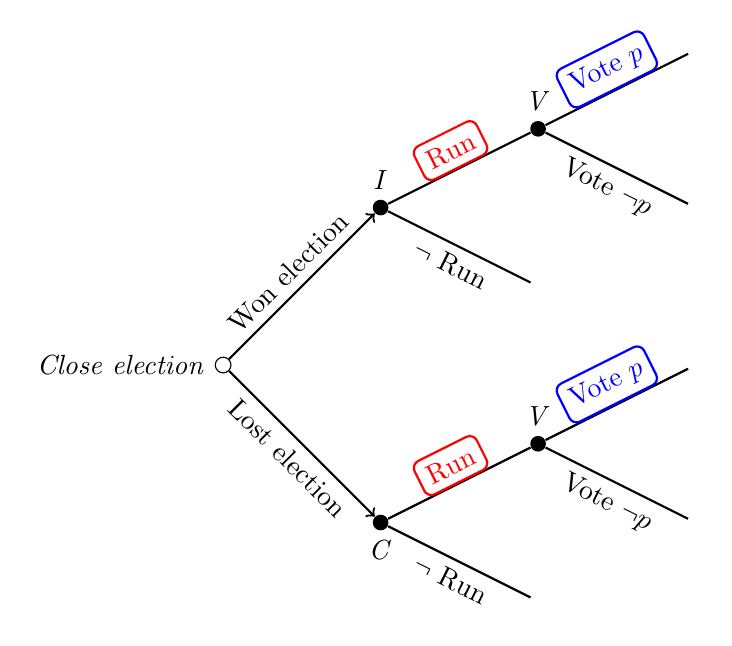
\begin{tikzpicture}[grow=right, sloped]

\node[circle, inner sep = 2, draw, label = left:\emph{Close election}] at (0,0) (a){};
\node[circle, inner sep = 2, fill = black, label = \emph{I}] at (2,2)(b){};
\node[circle, inner sep = 2, fill = black, label = below:\emph{C}] at (2,-2)(c){};
\path[->,draw,thick]
    (a) edge node [above] {Won election} (b)
    (a) edge node [below] {Lost election} (c);
\node[circle, inner sep = 2, fill = black, label = \emph{V}] at (4,3)(d){};
\node[circle, inner sep = 2] at (4,1)(e){};
\node[circle, inner sep = 2, fill = black, label = \emph{V}] at (4,-1)(f){};
\node[circle, inner sep = 2] at (4,-3)(g){};
\path[-,draw,thick]
    (b) edge node [above, draw, color = red, rounded corners = 1mm] {Run} (d)
    (b) edge node [below] {$\neg$ Run} (e)
    (c) edge node [above, draw, color = red, rounded corners = 1mm] {Run} (f)
    (c) edge node [below] {$\neg$ Run} (g);
\node[circle, inner sep = 2] at (6,4)(h){};
\node[circle, inner sep = 2] at (6,2)(i){};
\node[circle, inner sep = 2] at (6,0)(j){};
\node[circle, inner sep = 2] at (6,-2)(k){};
\path[-,draw,thick]
    (d) edge node [above, draw, color = blue, rounded corners = 1mm] {Vote $p$} (h)
    (d) edge node [below] {Vote $\neg p$ } (i)
    (f) edge node [above, draw, color = blue, rounded corners = 1mm] {Vote $p$} (j)
    (f) edge node [below] {Vote $\neg p$} (k);


\end{tikzpicture}
\caption{Sequence of actions in electoral RD study of disincumbency advantage.}\label{fig:rd}
\end{figure}

\citet{klasnjatitiunik2017} advocate imputing a 0 outcome when a party does not run in $t+1$ to measure the ``unconditional'' effect of incumbency. This decomposition suggests that the constituent quantities $ E[\text{Ran}_p|Z = z]$ and $E[\text{MoV}_p|\text{Ran}_p = 1, Z = z]$ should \emph{also} be of interest. Differences in these quantities define three estimands of interest:
\begin{enumerate}
\item $LATE$ on unconditional electoral outcomes (with 0's imputed when a party does not run).
\begin{align*}
LATE_{UC} &= \lim_{x \downarrow c}E[Y_p] -\lim_{x \uparrow c}E[Y_p] \\
\end{align*}
\item $LATE$ on party $p$ running in election $t+1$.
\begin{align*}
LATE_{Ran} &=  \lim_{x \downarrow c}E[Ran_p] -\lim_{x \uparrow c}E[Ran_p] 
\end{align*}
\item Post-treatment estimand measuring electoral outcomes given that the party runs in election $t+1$.
\begin{align*}
PT_{Y} &=  \lim_{x \downarrow c}E[Y_p|Ran_p] -\lim_{x \uparrow c}E[Y_p|Ran_p] 
\end{align*}

In Figure \ref{fig:rdd}, the left column of panels reports estimates of the unconditional LATE on re-election ($LATE_{UC}$), by quantile of bureaucratic quality. The next column of panels reports estimates of the $LATE_{Ran}$, by quantiile of bureaucratic quality. The third and right columns report $PT_Y$ for two operationalizations of $Y$: a binary indicator for won, and margin of victory (or defeat) of the incumbent candidate. 
\end{enumerate}



\subsection{Design validation, robustness}

In Table \ref{tab:mccrary}, I test for differential sorting (or differential density) around the electoral cutoff within each of the bins of bureaucratic quality using the test proposed by \citet{mccrary2008}. I find no evidence of differential sorting.

\begin{table}[h]
\centering
\input{TABLES/rdd_mccrary}
\caption{\citet{mccrary2008} tests for sorting in the running variable for each subgroup in the analysis. The $Z$-statistic is the test statistic. The $p$-value tests the null hypothesis of no sorting at the threshold.}\label{tab:mccrary}
\end{table}

In Figure \ref{fig:rddrobust}, I report analogous specifications to Figure \ref{fig:rdd} varying the bandwith selection for the regression discontinuity sample and the kernel employed by the \citet{calonicoetal2014} estimator. 

\begin{figure}
\resizebox{\textwidth}{!}{\includegraphics{FIGUREs/rdd_plot_robust.pdf}}
\caption{This figure replicates Figure \ref{fig:rdd} with alternative bandwidth selection (from each sample versus from the pooled sample) and kernels (triangular vs. uniform). Note that Figure \ref{fig:rdd} utilizes the bandwidth from the full, pooled sample with a triangular kernal.}\label{fig:rddrobust}
\end{figure}

\clearpage
\begin{comment}
\section{Effects of Information Provision}


\subsection{Corruption and electoral performance in the sample}
Table \ref{tab:result4a} replicates \citet{ferrazfinan2008} for the sample of audited municipalities with an incumbent running. Consistent with that paper, electoral performance is decreasing in corruption. Note that this table is intended only to demonstrate that the sign of the association between (endogenous) corruption and vote share is consistent with predictions.
\begin{table}
\centering
\input{TABLES/result4a}
\caption{Replication of \citet{ferrazfinan2008} for the audited municipalities with an incumbent running for re-election using the corruption metrics used in this paper.}\label{tab:result4a}
\end{table}


\subsection{Bureaucratic quality and electoral performance of incumbents}
Table \ref{tab:result4b} examines the relationship between bureaucratic quality and re-election. I find modest evidence that incumbents in places with higher levels of bureaucratic quality perform better consistent with the idea that any incumbency disadvantage occurs in lower quantiles of the sample. The difference in vote share is generally better powered than the binary indicator for re-election. 
\begin{table}
\centering
\input{TABLES/result4b}
\caption{Bureaucratic quality and electoral performance among municipalities with an incumbent running.}\label{tab:result4b}
\end{table}

\subsection{The effect of information}

Here, we are interested in the effect of being audited (regardless of the outcome of the audit) on the probability of re-election. Denoting re-election by $R \in \{0,1\}$ and assignment to a randomized audits as $Z = 1$, the ATE is defined as:
\begin{align*}
E[R|Z=1] - E[R|Z=0]
\end{align*}

I provide a slight adaption to the model to account for the research design introduced by the audits. I assume that after voters observe (resp. does not observe $g_1$), they probabilistically receive another signal that reveals the politician's allocation if assigned to treatment, $Z = 1$. Specifically, with probability $p_n$, citizens observe the signal realization $N$ via observation of public goods per the model characterized in Proposition \ref{prop1}. When assigned to treatment, with probability $p_a$, a citizen observes the realization $A \in \{0,1\}$, which is given by an exogenous report of the politician's first period allocation $a_1 \in \{0, 1\}$. I assume that $N \perp A$. I assume that the prior may be heterogeneous, but is an accurate assessment of the proportion of types in the candidate pool. \\ 

Consider the four cases of the Equilibrium in Proposition \ref{prop1}:
\begin{itemize}
	\item $q < \frac{1}{\overline{\theta}}$: Here, the posterior belief, upon realization of $N$ is $\mu = \pi$. Upon realization of $A$, the posterior belief is similarly $\mu = \pi$. It is thus trivial to show that:
\begin{align*}
E[R|Z=1]&= 
\begin{aligned}
\int_\pi \big[&\pi \left(p_a p_n \tau(\pi, \boldsymbol{a}) + p_a (1-p_n) \tau(\pi, \boldsymbol{a}) + p_n(1-p_a)\tau(\pi, \boldsymbol{a}) + (1-p_a)(1-p_n)\tau(\pi, \boldsymbol{a})\right)  +\\
&(1-\pi)\left(p_a p_n \tau(\pi, \boldsymbol{a}) + p_a (1-p_n) \tau(\pi, \boldsymbol{a}) + p_n(1-p_a)\tau(\pi, \boldsymbol{a}) + (1-p_a)(1-p_n)\tau(\pi, \boldsymbol{a})\right)\big] d\pi \\
\end{aligned}
&=\int_\pi \tau(\pi, \boldsymbol{a}) d\pi\\
&= \frac{1}{2} \\
E[R|Z=0] &= \pi \left( p_n \tau(\pi, \boldsymbol{a}) +  (1-p_n) \tau(\pi, \boldsymbol{a})\right) + (1-\pi)\left(p_n \tau(\pi, \boldsymbol{a}) + (1-p_n)\tau(\pi, \boldsymbol{a})\right) d\pi 
 \\
&=\int_\pi \tau(\pi, \boldsymbol{a}) d\pi\\
&= \frac{1}{2} \\
\end{align*}

\item $q \in [\frac{1}{\overline{\theta}}, \frac{2b (1 - \pi \overline{\theta})}{\underline{\theta}(2b (1-\pi \overline{\theta}) + p\overline{\theta}(1 - \pi))})$: Here, the posterior belief upon realization of $N$ is $\mu = 1$ if public goods are observed, and $\mu = \frac{\pi (1-\overline{\theta})}{\pi(1-\overline{\theta}) + 1-\pi}$ if public goods are not observed. The posterior beliefs upon realization of $A$ are $\mu =  1$ if $a =1$  and $\mu = 0$ if $a=0$. 
\begin{align*}
E[R|Z=1] &= \begin{aligned}\int_\pi
\big[ &\pi \big(p_a \tau(1, \boldsymbol{a})  +p_n(1-p_a)\overline{\theta} \tau(1, \boldsymbol{a}) + p_n(1-p_a)(1-\overline{\theta}) \tau(\frac{\pi (1-\overline{\theta})}{\pi(1-\overline{\theta}) + 1-\pi}, \boldsymbol{a}) + \\
&(1-p_n)(1-p_a)\tau(\pi, \boldsymbol{a})\big) + \\
&(1-\pi)\big(p_a \tau(0, \boldsymbol{a}) + (1-p_a)p_n\tau(\frac{\pi (1-\overline{\theta})}{\pi(1-\overline{\theta}) + 1-\pi}, \boldsymbol{a}) + (1-p_a)(1-p_n)\tau(\pi, \boldsymbol{a}) \big)\big]d\pi
\end{aligned} \\
&= \frac{1}{2}\\
E[R|Z=0] &= \begin{aligned}\int_\pi
\big[ &\pi \big(p_n\overline{\theta} \tau(1, \boldsymbol{a}) + p_n(1-\overline{\theta}) \tau(\frac{\pi (1-\overline{\theta})}{\pi(1-\overline{\theta}) + 1-\pi}, \boldsymbol{a}) + (1-p_n)\tau(\pi, \boldsymbol{a})\big) + \\
&(1-\pi)\big(p_n\tau(\frac{\pi (1-\overline{\theta})}{\pi(1-\overline{\theta}) + 1-\pi}, \boldsymbol{a}) + (1-p_n)\tau(\pi, \boldsymbol{a}) \big)\big]d\pi
\end{aligned} \\
&= \frac{1}{2}
\end{align*}
\item $q \in \left[ \max\{\frac{1}{\overline{\theta}},\frac{2b (1 - \pi \overline{\theta})}{\underline{\theta}(2b (1-\pi \overline{\theta}) + p\overline{\theta}(1 - \pi))}\}, \frac{1}{\underline{\theta}}\right)$: In this region, the posterior belief upon realization of $N$ is $\mu = \frac{\pi \overline{\theta}}{\pi \overline{\theta} +(1-\pi)\underline{\theta}}$ if public goods are observed, and $\mu = \frac{\pi (1-\overline{\theta})}{\pi(1-\overline{\theta})+(1-\pi)(1-\underline{\theta})}$ if public goods are not observed. Realization of $A$ provides no additional information since both types allocate to public goods, so the posterior is equivalent to the prior (if $N$ is not realized) or the posterior (if $N$ is realized). Note that in this case, $\tau(\cdot)$ accounts for the fact that the incompetent type will shirk in the second period. 
\begin{align*}
E[R|Z=1] &= \begin{aligned}\int_\pi
\big[ &\pi \big(p_n \overline{\theta} \tau(\frac{\pi \overline{\theta}}{\pi \overline{\theta} +(1-\pi)\underline{\theta}}, \boldsymbol{a})  +p_n(1-\overline{\theta}) \tau(\frac{\pi (1-\overline{\theta})}{\pi(1-\overline{\theta})+(1-\pi)(1-\underline{\theta})}, \boldsymbol{a}) + \\
&(1-p_n)\tau(\pi, \boldsymbol{a})\big) + (1-\pi)\big(p_n \underline{\theta} \tau(\frac{\pi \overline{\theta}}{\pi \overline{\theta} +(1-\pi)\underline{\theta}}, \boldsymbol{a})  +\\
&p_n(1-\underline{\theta}) \tau(\frac{\pi (1-\overline{\theta})}{\pi(1-\overline{\theta})+(1-\pi)(1-\underline{\theta})}, \boldsymbol{a}) + (1-p_n) \tau(\pi, \boldsymbol{a})\big) \big] d\pi
\end{aligned} \\
 &= \int_\pi \frac{b- \underline{\theta} q(1-\pi)}{2b} d\pi = \frac{(2b -\underline{\theta}q(2-\pi))\pi}{4b}\\
E[R|Z=0] &= \begin{aligned}\int_\pi
\big[ &\pi \big(p_n \overline{\theta} \tau(\frac{\pi \overline{\theta}}{\pi \overline{\theta} +(1-\pi)\underline{\theta}}, \boldsymbol{a})  +p_n(1-\overline{\theta}) \tau(\frac{\pi (1-\overline{\theta})}{\pi(1-\overline{\theta})+(1-\pi)(1-\underline{\theta})}, \boldsymbol{a}) + \\
&(1-p_n)\tau(\pi, \boldsymbol{a})\big) + (1-\pi)\big(p_n \underline{\theta} \tau(\frac{\pi \overline{\theta}}{\pi \overline{\theta} +(1-\pi)\underline{\theta}}, \boldsymbol{a})  +\\
&p_n(1-\underline{\theta}) \tau(\frac{\pi (1-\overline{\theta})}{\pi(1-\overline{\theta})+(1-\pi)(1-\underline{\theta})}, \boldsymbol{a}) + (1-p_n) \tau(\pi, \boldsymbol{a})\big) \big] d\pi
\end{aligned} \\
&= \int_\pi \frac{b- \underline{\theta} q(1-\pi)}{2b} d\pi = \frac{(2b -\underline{\theta}q(2-\pi))\pi}{4b}\\
\end{align*}
\item $q \geq \frac{1}{\underline{\theta}}$. In this region, the posterior belief upon realization of $N$ is $\mu = \frac{\pi \overline{\theta}}{\pi \overline{\theta} +(1-\pi)\underline{\theta}}$ if public goods are observed, and $\mu = \frac{\pi (1-\overline{\theta})}{\pi(1-\overline{\theta})+(1-\pi)(1-\underline{\theta})}$ if public goods are not observed. Realization of $A$ provides no additional information since both types allocate to public goods, so the posterior is equivalent to the prior (if $N$ is not realized) or the posterior (if $N$ is realized). This differs by from the previous case in the second period allocation of the incompetent type, which enters in $\tau(\cdot)$.
\begin{align*}
E[R|Z=1] &= \begin{aligned}\int_\pi
\big[ &\pi \big(p_n \overline{\theta} \tau(\frac{\pi \overline{\theta}}{\pi \overline{\theta} +(1-\pi)\underline{\theta}}, \boldsymbol{a})  +p_n(1-\overline{\theta}) \tau(\frac{\pi (1-\overline{\theta})}{\pi(1-\overline{\theta})+(1-\pi)(1-\underline{\theta})}, \boldsymbol{a}) + \\
&(1-p_n)\tau(\pi, \boldsymbol{a})\big) + (1-\pi)\big(p_n \underline{\theta} \tau(\frac{\pi \overline{\theta}}{\pi \overline{\theta} +(1-\pi)\underline{\theta}}, \boldsymbol{a})  +\\
&p_n(1-\underline{\theta}) \tau(\frac{\pi (1-\overline{\theta})}{\pi(1-\overline{\theta})+(1-\pi)(1-\underline{\theta})}, \boldsymbol{a}) + (1-p_n) \tau(\pi, \boldsymbol{a})\big) \big] d\pi
\end{aligned} \\
&= \frac{1}{2}\\
E[R|Z=0] &= \begin{aligned}\int_\pi
\big[ &\pi \big(p_n \overline{\theta} \tau(\frac{\pi \overline{\theta}}{\pi \overline{\theta} +(1-\pi)\underline{\theta}}, \boldsymbol{a})  +p_n(1-\overline{\theta}) \tau(\frac{\pi (1-\overline{\theta})}{\pi(1-\overline{\theta})+(1-\pi)(1-\underline{\theta})}, \boldsymbol{a}) + \\
&(1-p_n)\tau(\pi, \boldsymbol{a})\big) + (1-\pi)\big(p_n \underline{\theta} \tau(\frac{\pi \overline{\theta}}{\pi \overline{\theta} +(1-\pi)\underline{\theta}}, \boldsymbol{a})  +\\
&p_n(1-\underline{\theta}) \tau(\frac{\pi (1-\overline{\theta})}{\pi(1-\overline{\theta})+(1-\pi)(1-\underline{\theta})}, \boldsymbol{a}) + (1-p_n) \tau(\pi, \boldsymbol{a})\big) \big] d\pi
\end{aligned} \\
&= \frac{1}{2}\\
\end{align*}
\end{itemize}

First, I show that there is no evidence that incumbents in audited and un-audited municipalities run at different rates in Table \ref{tab:balance}. Because the audits were rolled out in sequential waves (lotteries), I also estimate marginal effects of each lottery round (each municipality was audited only once) to ensure that the decision the ATE is not obscuring heterogeneity as a function of audit timing. All models include state fixed effects because each lottery effectively blocked on state and the sample comprises all municipalities with a population under 450,000. Following \citet{hartmanhidalgo2018}, a two one-sided $t$-test test rejects the null hypothesis of that $ |ATE| \geq\pm 0.36\sigma$ at $p < 0.001$, where $\sigma$ is the variance of the outcome. \\


\begin{table}
\centering
\input{TABLES/bal_audits}
\caption{This table examines whether audited incumbents contest re-election at a differential rate than unaudited incumbents. Column 1 examines the ATE of audits on contesting re-election. Column 2 estimates the marginal effects of auditing in each round (a measure of treatment timing). The unit is the municipality. Heteroskedasticity-robust standard errors in parentheses.} \label{tab:balance}
\end{table}

To examine evidence that the ATE of audits on incumbent electoral performance, I employ equivalence testing as in \citet{hartmanhidalgo2018}. The theoretical prediction is that $ATE = 0$, so a traditional null hypothesis is an inappropriate test of the prediction. As such, I test the evidence against a null of an $|ATE| \geq  0.36 \sigma$, a hypothesis recommended by \citet{hartmanhidalgo2018}. I examine both raw (i.e. difference-in-means) and covariate-adjusted specifications. In principle, covariate-adjustment is needed to adjust for the blocking randomization strategy used in the CGU lotteries. I use two electoral dependent variables: an indicator for re-election and change in incumbent vote-share. \\

\begin{figure}
\centering
\includegraphics{FIGUREs/equiv_tests.pdf}
\caption{Visualizations of two one-sided T-tests. The top panel presents the omnibus test across all municipalities where an incumbent contested re-election in 2004, $N =2228$. The bottom three panels disaggregate by tercile. Points represent the standardized estimated ATE. The gray rectangles correspond to the inverted equivalence range that is ascertained from the data. The vertical lines represent the null hypothesis against which I am testing.}\label{fig:equiv}
\end{figure}

Figure \ref{fig:equiv} rejects the null hypothesis of $|ATE| \geq 0.36\sigma$ at the $p < 0.005$ level in all specifications. We reject this null for all subsamples of bureaucratic quality except for the ``re-elected'' outcome in Tercile 2. Note however, that the power of the test is limited (analytically 0.63) for this specification. Moreover, there is no evidence of such an effect on change in vote share in the same tercile. This provides one way to test the prediction of an ATE of 0 in a frequentist framework.\footnote{An alternate test would use permutation tests/randomization inference. However, the assumption of a constant treatment effect for all units is inconsistent with this setting or the data where we expect (and \citet{ferrazfinan2008} find) evidence of heterogeneity.}

\clearpage
\end{comment}
\section{Existing studies of information and accountability}
I identify 16 studies examining information and accountability for the purposes of Figure \ref{fig_qog}. Table \ref{tab:info_account} provides the relevant citations.
\begin{table}[H]
\resizebox{\textwidth}{!}{
\centering
	\begin{tabular}{clp{7cm}ccc} \hline
	& Country & Citation & Design & Metaketa-I &Included in Fig. \ref{fig_meta} \\ \hline \hline
	1& Benin & \citet{adidaetal2017} & E & $\checkmark$ & $\checkmark$\\
	2& Brazil &\citet{ferrazfinan2008} & NE & & \\
	3& Brazil & \citet{boasetal2018} & E & $\checkmark$ & $\checkmark$\\
	4& Burkina Faso & \citet{lierlholmlund2017} & E & $\checkmark$ & $\checkmark$\\
	5& India & \citet{banerjeeetal2011}& E & &$\checkmark$\\ 
	6& India & \citet{georgeetal2018} & E &&$\checkmark$\\ 
	7& Philippines & \citet{cruzetal2019b} & E & &\\
	8& Philippines & \citet{cruzetal2019a} & E & &$\checkmark$\\
	9& Mexico & \citet{chong2015} & E & &$\checkmark$\\
	10& Mexico & \citet{ariasetal2019} & E& $\checkmark$&$\checkmark$ \\
	11& Mexico & \citet{enriquez2019} & E& &$\checkmark$\\
	12& Mexico & \citet{larreguyetal2020} &NE &\\
	13& Senegal & \citet{bhandarietal2019} & E & &$\checkmark$\\
	14& Uganda & \citet{humphreysweinstein2012} & E& &\\
	15& Uganda & \citet{buntaineetal2018} & E & $\checkmark$& $\checkmark$\\
	16& Uganda & \citet{platasraffler2019} & E & $\checkmark$&$\checkmark$\\ \hline 

	\end{tabular}}
\caption{Studies of information and accountability and their locations. Under design, ``E'' corresponds to an experiment and ``NE'' corresponds to a natural experiment (one where the investigators did not manipulate provision of information).}\label{tab:info_account}
\end{table}
\clearpage
\singlespacing
\bibliographystyle{apsr2}
\bibliography{dissbib}
\end{document}

\end{document}